\subsection{豪斯多夫空间}

命题 1. 设 X 是一个拓扑空间。则下列命题等价：

\begin{enumerate}
\def\labelenumi{(\Alph{enumi})}
\setcounter{enumi}{7}
\tightlist
\item
  X 的任意两个不同的点都有不相交的邻域。
\end{enumerate}

(Hi) X 的任意一点的闭邻域之交仅由该点组成。

(Hii) 积空间 \(\mathbf{X} \times \mathbf{X}\) 的对角线是闭集。

(Hiii) 对每个集合 I，积空间 Y = X \(^{I}\) 的对角线在 Y 中是闭集。

\((\mathbf{H}^{\mathrm{iv}})\) \(\mathbf{X}\) 上没有滤子具有多于一个的极限点。

(Hv) 若 X 上的滤子 \(\mathfrak{F}\) 收敛于 \(x\)，则 \(x\) 是 \(\mathfrak{F}\) 的唯一聚点。

我们将证明蕴涵关系

以及

\[
\begin{array}{r l} (\mathrm{H}) & \Longrightarrow (\mathrm{H} ^ {\mathrm{i}}) \Longrightarrow (\mathrm{H} ^ {\mathrm{v}}) \Longrightarrow (\mathrm{H} ^ {\mathrm{iv}}) \Longrightarrow (\mathrm{H}) \\ (\mathrm{H}) & \Longrightarrow (\mathrm{H} ^ {\mathrm{iii}}) \Longrightarrow (\mathrm{H} ^ {\mathrm{ii}}) \Longrightarrow (\mathrm{H}). \end{array}
\]

\((\mathrm{H}) \Longrightarrow (\mathrm{H}^{\mathrm{i}}): \text{若 } x \neq y \text{，则存在一个开邻域 } \mathrm{U} \text{，包含 } x \text{，以及一个开邻域 } \mathrm{V} \text{，包含 } y \text{，使得 } \mathrm{U} \cap \mathrm{V} = \varnothing; \text{因此 } y \notin \overline{\mathrm{U}}.\)

\((\mathbf{H}^{\mathrm{i}}) \Longrightarrow (\mathbf{H}^{\mathrm{v}}): \text{令 } y \neq x; \text{则存在一个闭邻域 } V \text{，包含 } x \text{，使得 } y \notin V, \text{且根据假设存在 } M \in \mathfrak{F} \text{使得 } M \subset V; \text{故 } M \cap \mathbb{C}V = \emptyset. \text{但是 } \mathbb{C}V \text{是一个邻域，其中包含 } y; \text{故 } y \text{对滤子而言不是聚点，滤子为 } \mathfrak{F}.\)

\((\mathbf{H}^{\mathrm{v}}) \Rightarrow (\mathbf{H}^{\mathrm{iv}})\)：显然，因为滤子的每个极限点也是聚点。

\((\mathrm{H}^{\mathrm{iv}}) \Longrightarrow (\mathrm{H})\)：设 \(x \neq y\)，且任何邻域 \(V\)（即 \(x\) 的邻域）与任何邻域 \(W\)（即 \(y\) 的邻域）相交。于是诸集合 \(V \cap W\) 构成一个滤子的基，该滤子以 \(x\) 与 \(y\) 两者为极限点，这与假设矛盾。

\((\mathrm{H}) \Longrightarrow (\mathrm{H}^{\mathrm{iii}})\)：设 \((x) = (x_{\iota})\) 是 \(\mathbf{X}^{\mathbf{I}}\) 中不属于对角线 \(\Delta\) 的一点。则至少存在两个指标 \(\lambda, \mu\) 使 \(x_{\lambda} \neq x_{\mu}\)。设 \(\mathbf{V}_{\lambda}\)（相应地，\(\mathbf{V}_{\mu}\)）是 \(x_{\lambda}\)（相应地，\(x_{\mu}\)）在 \(\mathbf{X}\) 中的一个邻域，使得 \(\mathbf{V}_{\lambda} \cap \mathbf{V}_{\mu} = \emptyset\)；则集合 \(W = V_{\lambda} \times V_{\mu} \times \prod_{\iota \neq \lambda, \mu} X_{\iota}\)（其中 \(X_{\iota} = X\)，\(\iota \neq \lambda, \mu\)）是 \(x\) 在 \(X^{\mathbf{I}}\) 中的一个邻域（\(\S 4, no.1\)），且不与 \(\Delta\) 相交。因此 \(\Delta\) 在 \(X^{\mathbf{I}}\) 中是闭集。

\((\mathbf{H}^{\mathrm{iii}}) \Rightarrow (\mathbf{H}^{\mathrm{ii}}): \text{显然。}\)

\((H^{ii}) \Longrightarrow (H)\)：若 \(x \neq y\)，则 \((x, y) \in X \times X\) 不属于对角线 \(\Delta\)，因此（§ 4，第 1 目）存在邻域 \(V\)（即 \(x\) 的邻域）与邻域 \(W\)（即 \(y\) 的邻域），都在 \(X\) 中，使得 \((V \times W) \cap \Delta = \emptyset\)，这就意味着

\[
\mathbf {V} \cap \mathbf {W} = \varnothing .
\]

定义 1. 满足命题 1 中诸条件的拓扑空间称为豪斯多夫空间或分离空间；这种空间的拓扑称为豪斯多夫拓扑。

公理 (H) 称为豪斯多夫公理。

例. 任何离散空间都是豪斯多夫的。有理直线 Q 是豪斯多夫的，因为若 x, y 是两个有理数且 x \textless{} y，则存在有理数 z 使得 x \textless{} z \textless{} y，而 x 的邻域 {]}\(\leftarrow\) , z{[} 与 y 的邻域 {]}z, \(\rightarrow\) {[} 不相交。

一个至少含有两个点且带有最粗拓扑（§ 2，第 2 目）的集合 X 不是豪斯多夫空间。

设 \(f: X \to Y\) 是集合 \(X\) 到豪斯多夫空间 \(Y\) 中的一个映射；则由命题 1 立即得出，\(f\) 关于滤子 \(\mathfrak{F}\)（\(X\) 上的）至多有一个极限，且若 \(f\) 以 \(y\) 为关于 \(\mathfrak{F}\) 的极限，则 \(y\) 是 \(f\) 关于 \(\mathfrak{F}\) 的唯一聚点。

命题 2. 设 \(f, g\) 是拓扑空间 \(\mathbf{X}\) 到豪斯多夫空间 \(\mathbf{Y}\) 中的两个连续映射；则 \(x \in \mathbf{X}\) 且 \(f(x) = g(x)\) 的点全体组成 \(\mathbf{X}\) 中的一个闭集。

因为这个集合是 \(\mathbf{Y} \times \mathbf{Y}\) 的对角线在映射 \(x \to (f(x), g(x))\) 下的逆像，而该映射是连续的（\(\S 4\)，第 1 目，命题 1）。因此结论由 (H \(^{ii}\) ) 与 \(\S 2\)，第 1 目，定理 1 得出。

推论 1（恒等延拓原理）. 设 \(f, g\) 是拓扑空间 \(X\) 到豪斯多夫空间 \(Y\) 中的两个连续映射。若 \(f(x) = g(x)\) 在 \(X\) 的一个稠密子集的所有点处成立，则 \(f = g\)。

换句话说，X 到 Y（豪斯多夫）中的一个连续映射由它在 X 的一个稠密子集的所有点处的值唯一确定。

推论 2. 若 \(f\) 是拓扑空间 \(\mathbf{X}\) 到豪斯多夫空间 \(\mathbf{Y}\) 中的一个连续映射，则 \(f\) 的图象在 \(\mathbf{X} \times \mathbf{Y}\) 中是闭集。

因为这个图象是由所有 \((x, y) \in \mathbf{X} \times \mathbf{Y}\)（其中 \(f(x) = y\)）组成的集合，而两个映射 \((x, y) \to y\) 与 \((x, y) \to f(x)\) 都是连续的。

命题 3. 设 \((x_{i})_{1\leqslant i\leqslant n}\) 是豪斯多夫空间 \(\mathbf{X}\) 中互不相同的点组成的一个有限族；则每个 \(x_{i}\) 有一个邻域 \(\mathbf{V}_{i}\)（\(\mathbf{X}\) 中的），使得诸 \(\mathbf{V}_{i}\)（\(1\leqslant i\leqslant n\)）两两不相交。

证明对 \(n\) 用归纳法：\(n = 2\) 的情形就是公理 (H)。于是设 \(W_i\)（\(1 \leqslant i \leqslant n - 1\)）是 \(x_i\) 的邻域，使诸 \(W_i\) 两两不相交。另一方面，对 \(1 \leqslant i \leqslant n - 1\)，存在邻域 \(T_i\)（即 \(x_i\) 的邻域）与邻域 \(U_i\)（即 \(x_n\) 的邻域），二者不相交。若取 \(V_i\) 为 \(W_i \cap T_i\)（\(1 \leqslant i \leqslant n - 1\)），并取

\[
\mathrm{V} _ {n} = \bigcap_ {i = 1} ^ {n - 1} \mathrm{U} _ {i},
\]

则命题的条件即告满足。

推论. 每个有限豪斯多夫空间都是离散的。

命题 4. 豪斯多夫空间的每个有限子集都是闭集。

因为每个由单点组成的子集都依据公理 (H \(^{i}\) ) 是闭集。

命题 5. 设 X 是一个拓扑空间，并设对 X 的每对不同的点 x, y，都存在 X 到豪斯多夫空间 \(X'\) 中的一个连续映射 f，使得 \(f(x) \neq f(y)\)。则 X 是豪斯多夫的。

设 \(V'\) 与 \(W'\) 分别是 \(f(x)\) 与 \(f(y)\) 在 \(X'\) 中的不相交邻域；则 \(\overline{f}^1(V')\) 与 \(\overline{f}^1(W')\) 分别是 \(x\) 与 \(y\) 在 \(X\) 中的不相交邻域。

推论. 每个比豪斯多夫拓扑更细的拓扑都是豪斯多夫的。

\subsection{豪斯多夫空间的子空间与积}

豪斯多夫空间 X 的子空间 A 是豪斯多夫的，这可由把第 1 目命题 5 应用于典范单射 A → X 看出。反之，我们有

命题 6. 若拓扑空间 X 的每一点都有一个闭邻域，它是 X 的豪斯多夫子空间，则 X 是豪斯多夫的。

设 \(x \in X\)，并设 \(V\) 是 \(x\) 在 \(X\) 中的一个闭邻域，使得子空间 \(V\) 是豪斯多夫的。则 \(x\) 在 \(V\) 中的诸闭邻域之交为 \(\{x\}\)（公理 \((H^i)\)）；但它们也是 \(x\) 在 \(X\) 中的闭邻域（\(\S 3, no. 1\)），因此 \(X\) 满足 \((H^i)\)。

\pandocbounded{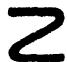
\includegraphics[keepaspectratio]{images/part001_a9a6e172.jpg}}

存在这样的非豪斯多夫空间，其中每一点都有一个豪斯多夫邻域（习题 7）。

命题 7. 豪斯多夫空间的每个积都是豪斯多夫的。反之，若非空空间的积是豪斯多夫的，则每个因子都是豪斯多夫空间。

设 \(X = \prod_{i \in I} X_i\) 是拓扑空间的一个积。于是，若 \(x, y\) 是 \(X\) 的两个不同的点，则 \(\text{pr}_i x \neq \text{pr}_i y\) 对某个指标 \(i\) 成立，而第 1 目命题 5 表明，\(X\) 是豪斯多夫的，只要诸 \(X_i\) 是豪斯多夫的。反之，若 \(X\) 是豪斯多夫的且诸 \(X_i\) 非空，则每个 \(X_i\) 同胚于 \(X\) 的一个子空间（\(\S 4\)，第 2 目，命题 4），因而是豪斯多夫的。

推论 1. 设 X 是一个集合，\((\mathbf{Y}_{\iota})_{\iota \in \mathbf{I}}\) 是豪斯多夫拓扑空间的一个族，且对每个 \(\iota \in I\)，设 \(f_{\iota}\) 是 X 到 \(Y_{\iota}\) 中的一个映射。设 X 带有最粗拓扑 \(\mathfrak{T}\)，使诸 \(f_{\iota}\) 连续。则 X 为豪斯多夫的一个必要充分条件是：对 X 的每对不同的点 x, y，\(f_{\iota}(x) \neq f_{\iota}(y)\) 对某个指标 \(\iota \in I\) 成立。

该条件依据第 1 目命题 5 是充分的。反之，设 X 是豪斯多夫的；令 \(Y = \prod_{\iota \in I} Y_{\iota}\)，并令 \(f = (f_{\iota})_{\iota \in I}\) 为映射 \(x \to (f_{\iota}(x))\)。由上面的命题 7，Y 是豪斯多夫的；又由 §4 第 1 目命题 3，\(\mathfrak{T}\) 是 Y 的拓扑在 f 下的逆像。若对 X 的两个不同的点 x, y 有 \(f(x) = f(y)\)，则显然每个（拓扑 \(\mathfrak{T}\) 中的）包含 x 的开集也包含 y，这与 X 是豪斯多夫的假设相矛盾。

推论 2. 设 \((\mathbf{X}_{\alpha}, f_{\alpha \beta})\) 是拓扑空间的一个逆系统。若诸 \(\mathbf{X}_{\alpha}\) 是豪斯多夫的，则 \(\mathbf{X} = \varprojlim \mathbf{X}_{\alpha}\) 是豪斯多夫的，并且是 \(\prod_{\alpha} \mathbf{X}_{\alpha}\) 的一个闭子空间。

第一个断言由 X 是豪斯多夫空间 \(\prod_{\alpha} X_{\alpha}\) 的子空间（命题 7）这一事实得出。为证 X 在积空间中是闭的，设 \(F_{\alpha\beta} (\alpha \leqslant \beta)\) 是 \(\prod_{\alpha} X_{\alpha}\) 中由使 \(\operatorname{pr}_{\alpha}x = f_{\alpha\beta}(\operatorname{pr}_{\beta}x)\) 的点 x 组成的子集；诸 \(F_{\alpha\beta}\) 在 \(\prod_{\alpha} X_{\alpha}\) 中是闭的（第 1 目，命题 2），因此它们的交 X 也是闭的。

显然，豪斯多夫空间的任意和（§ 2，第 4 目，例 3）都是豪斯多夫空间。

\subsection{豪斯多夫商空间}

我们来寻求使商空间 X/R 为豪斯多夫空间的条件（这时称等价关系 R 为豪斯多夫的）。首先，若 X/R 是豪斯多夫的，则 X/R 中由单点组成的诸子集是闭的（第 1 目，命题 4），因而每个模 R 的等价类在 X 中是闭的。但这个必要条件并不充分。

X/R 中开集的定义给出如下的必要充分条件：X/R 是豪斯多夫的，当且仅当 X 中任意两个不同的等价类都包含在 X 的两个不相交的饱和开子集中。我们将给出其他更便于使用的条件。

命题 8. 商空间 X/R 为豪斯多夫的一个必要条件是 R 的图象 C 在 X × X 中是闭的。若等价关系 R 是开的，则此条件也是充分的。

设 \(\varphi: X \to X/R\) 是典范映射；则 \(C\) 是 \(\varphi \times \varphi: X \times X \to (X/R) \times (X/R)\) 下对角线 \(\Delta\)（即 \((X/R) \times (X/R)\) 的对角线）的逆像。因此命题的第一部分由 \(\varphi \times \varphi\) 的连续性得出{[}公理 \((H^{ii})\) 及 §2 第 1 目定理 1{]}。若 \(R\) 是开的，则 \((X/R) \times (X/R)\) 可等同于商空间 \((X \times X)/(R \times R)\)（§5，第 3 目，命题 8 的推论），而 \(\Delta\) 这时等同于 \((X \times X)/(R \times R)\) 中集合 \(C\)（它关于 \(R \times R\) 是饱和的）的典范象。于是 \(\Delta\) 在 \(X \times X\) 中是闭的，从而 \(X\) 是豪斯多夫的。

\pandocbounded{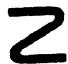
\includegraphics[keepaspectratio]{images/part001_7b053cb2.jpg}}

若 R 不是开的，则存在这样的例子：C 是闭的而 R 不是豪斯多夫的（习题 10 与 28）。

为证 X/R 是豪斯多夫的，我们也可以应用第 1 目命题 5：设 M 与 N 是 R 的两个不同的等价类，只需存在 X 的一个开子集 A 到豪斯多夫空间 \(X'\) 中的一个连续映射 f，其中 A 关于 R 饱和且包含 M 与 N，使得 1) f 在 A 所含的每个模 R 等价类上取常值，2) f 在 M 与 N 上取不同的值。因为既然 \(A/R_{A}\) 可等同于 X/R 的一个开子集（§ 3，第 6 目，命题 10，推论 1），我们就可以对由 f 诱导的映射 g: \(A/R_{A} \to X'\) 应用第 1 目命题 5，因为 g 是连续的（§ 3，第 4 目，命题 6）。

特别地：

命题 9. 若 \(f\) 是拓扑空间 \(\mathbf{X}\) 到豪斯多夫空间 \(\mathbf{X}'\) 中的一个连续映射，而 \(\mathbf{R}\) 是等价关系 \(f(x) = f(y)\)，则商空间 \(\mathbf{X} / \mathbf{R}\) 是豪斯多夫的。

命题 10. 若 X 是豪斯多夫空间，且 X 关于等价关系 R 有一个连续截面 s，则 X/R 是豪斯多夫的，且 s (X/R) 在 X 中是闭的。

因为（§ 3，第 5 目）X/R 同胚于 X 的子空间 \(s(\mathrm{X}/\mathrm{R})\)，后者是豪斯多夫的。此外，\(s(\mathrm{X}/\mathrm{R})\) 是由所有 \(x \in \mathbf{X}\) 中使 \(s(\varphi(x)) = x\) 的点组成的集合，其中 \(\varphi: \mathbf{X} \to \mathbf{X}/\mathbf{R}\) 是典范映射；因此第二个断言由第 1 目命题 2 得出。

\subsection{正则空间}

命题 11. 拓扑空间 X 的下列性质等价：

(O \(_{III}\) ) X 的任一点的诸闭邻域组成的集合是该点的一个基本邻域系。

\((O_{\mathrm{III}}^{\prime})\) 给定闭子集 \(\mathbf{F}\)（\(\mathbf{X}\) 的）与任一点 \(x \notin \mathbf{F}\)，存在 \(x\) 的一个邻域与 \(\mathbf{F}\) 的一个邻域，二者不相交。

\((\mathrm{O}_{\mathrm{III}}) \Longrightarrow (\mathrm{O}_{\mathrm{III}}^{\prime})\)：若 \(\mathbf{F}\) 是闭的且 \(x \notin \mathbf{F}\)，则存在一个闭邻域 \(\mathbf{V}\)（即 \(x\) 的闭邻域），它包含于邻域 \(\complement \mathbf{F}\)（即 \(x\) 的邻域）中；\(\mathbf{V}\) 与 \(\complement \mathbf{V}\) 分别是 \(x\) 与 \(\mathbf{F}\) 的邻域，且没有公共点。

\((\mathrm{O}_{\mathrm{III}}^{\prime}) \Longrightarrow (\mathrm{O}_{\mathrm{III}})\)：若 \(W\) 是 \(x \in X\) 的一个开邻域，则存在邻域 \(U\)（即 \(x\) 的邻域）与邻域 \(V\)（即 \(\complement W\) 的邻域），二者不相交，因此 \(\overline{U} \subset W\)。

定义 2. 拓扑空间称为正则的，如果它是豪斯多夫的且满足公理 (O \(_{III}\) )；这时它的拓扑称为正则拓扑。

离散空间是正则的。* 我们将在 § 9 中看到，每个局部紧空间（特别地，实直线 R）都是正则的。*

命题 12. 正则空间的每个子空间都是正则的。

设 A 是正则空间 X 的一个子空间。既然 X 是豪斯多夫的，A 亦然（第 2 目）；另一方面，点 \(x \in A\) 关于 A 的每个邻域都具有形状 \(V \cap A\)，其中 V 是 x 在 X 中的邻域。既然 X 是正则的，就存在 x 在 X 中的一个邻域 W，它在 X 中是闭的且包含于 V；于是 \(W \cap A\) 是 x 在 A 中的邻域，在 A 中是闭的且包含于 \(V \cap A\)。由此即得结论。反之：

命题 13. 若拓扑空间 X 的每一点 x 都有一个闭邻域，它是 X 的正则子空间，则 X 是正则的。

由第 2 目命题 6，X 是豪斯多夫的。设 x 是 X 的任一点，V 是 x 的一个闭的正则邻域。若 U 是 x 的包含于 V 中的任一邻域，则 U 是 x 关于 V 的邻域；于是由假设，存在 x 在 V 中的一个邻域 W，它在 V 中是闭的且包含于 U。但既然 V 是 x 在 X 中的邻域，W 就是 x 在 X 中的邻域；又既然 V 在 X 中是闭的，W 就在 X 中是闭的。

注. 1) 存在这样的非豪斯多夫空间，其中每一点都有一个正则邻域（习题 7）。

\begin{enumerate}
\def\labelenumi{\arabic{enumi})}
\setcounter{enumi}{1}
\item
  存在豪斯多夫但非正则的空间（习题 20）。
\item
  比正则拓扑更细的拓扑未必是正则的（习题 20）。
\end{enumerate}

\subsection{连续延拓；二重极限}

定理 1. 设 X 是一个拓扑空间，A 是 X 的一个稠密子集，\(f: \mathbf{A} \to \mathbf{Y}\) 是 A 到正则空间 Y 中的一个映射。\(f\) 可延拓为连续映射 \(\overline{f}: \mathbf{X} \to \mathbf{Y}\) 的一个必要充分条件是：对每个 \(x \in \mathbf{X}\)，\(f(y)\) 当 \(y\) 趋于 \(x\) 且保持属于 A 时在 Y 中趋于一个极限。这时连续延拓 \(\overline{f}\)（把 \(f\) 延拓到 X 上）是唯一的。

\(\vec{f}\) 的唯一性由恒等延拓原理（第 1 目，命题 2，推论 1）得出。显然该条件是必要的，因为若 \(\vec{f}\) 在 X 上连续，则对每个 \(x \in X\) 我们有

\[
\overline {{f}} (x) = \lim _ {y > x, y \in \mathbf {A}} \overline {{f}} (y) = \lim _ {y > x, y \in \mathbf {A}} f (y)
\]

（§ 7，第 5 目）。反之，设该条件成立，并定义

\[
\overline {{f}} (x) = \lim _ {y \rightarrow x, y \in \mathbf {A}} f (y)
\]

（对每个 \(x \in X\)）；\(\overline{f}(x)\) 是 Y 中一个完全确定的元素，因为 Y 是豪斯多夫的。我们必须证明 \(\overline{f}\) 在每个点 \(x \in X\) 处连续。于是设 \(V'\) 是 \(\overline{f}(x)\) 在 Y 中的一个闭邻域；则由假设，存在 x 在 X 中的一个开邻域 V，使得 \(f(V \cap A) \subset V'\)。既然 V 是它的每一点的邻域，我们就有

\[
\overline {{f}} (z) = \lim _ {y > z, y \in \mathrm{V} \cap \mathrm{A}} f (y)
\]

（对每个 \(z \in \mathbf{V}\)）；由此得出 \(\overline{f}(z) \in f(\mathbf{V} \cap \mathbf{A}) \subset \mathbf{V}'\)，因为 \(\mathbf{V}'\) 是闭的。于是结论由 \(f(x)\) 的诸闭邻域构成 \(f(x)\) 在 \(\mathbf{Y}\) 中的一个基本邻域系这一事实得出。

映射 \(\bar{f}\) 称为由 f 连续延拓到 X 上而得到的映射。

在定理 1 的陈述中，Y 是正则的这一假设不能减弱，除非对 X、A 或 f 附加额外的限制（习题 19）。

推论. 设 \(\mathfrak{F}_1\) 是集合 \(X_1\) 上的一个滤子，\(\mathfrak{F}_2\) 是集合 \(X_2\) 上的一个滤子；设 \(\mathfrak{F}_1 \times \mathfrak{F}_2\) 是 \(X = X_1 \times X_2\) 上的积滤子（§ 6，第 7 目），并设 \(f\) 是 \(X\) 到正则空间 \(Y\) 中的一个映射。假设

\begin{enumerate}
\def\labelenumi{\alph{enumi})}
\item
  \(\lim_{\mathfrak{F}_1\times \mathfrak{F}_2}f\) 存在。
\item
  \(\lim_{x_2, \mathfrak{F}_2} f(x_1, x_2) = g(x_1)\) 对所有 \(x_1 \in \mathbf{X}_1\) 存在。
\end{enumerate}

则 \(\lim_{x_1, \mathfrak{F}_1} g(x_1)\) 存在且等于 \(\lim_{\mathfrak{F}_1 \times \mathfrak{F}_2} f\)。

设 \(X_1' = X_1 \cup \{ \omega_1 \}\)（相应地，\(X_2' = X_2 \cup \{ \omega_2 \}\)）是伴随于滤子 \(\mathfrak{F}_1\)（相应地，\(\mathfrak{F}_2\)）的拓扑空间（§ 6，第 5 目，例）。在积空间 \(X' = X_1' \times X_2'\) 中，设 \(X''\) 是子空间 \(X_1 \times X_2'\) 与 \(\{ (\omega_1, \omega_2) \}\) 的并。显然 \(X\) 是 \(X''\) 的稠密子空间，且诸假设蕴含：\(f(y_1, y_2)\) 当 \((y_1, y_2)\) 趋于任一点 \((x_1, x_2)\)（在 \(X''\) 中）且保持属于 \(X\) 时趋于一个极限。于是由定理 1 得出 \(f\) 连续延拓到 \(X''\) 上的存在性。又因为 \((\omega_1, \omega_2)\) 属于 \(X_1 \times \{ \omega_2 \}\) 关于 \(X''\) 的闭包，结论立即得出（§ 7，第 5 目）。

\subsection{正则空间上的等价关系}

命题 14. 设 X 是正则空间，R 是 X 上的一个闭等价关系。则 R 在 X × X 中的图象 C 是闭的。

设 \((a, b)\) 是 \(X \times X\) 中属于 C 的闭包的一点，并设 V（相应地，W）是 \(a\) 的一个闭邻域（相应地，\(b\) 的一个邻域）；则存在一点 \((x, y) \in C \cap (V \times W)\)。既然 \(x \in V\)，\(y\) 就属于 V 关于 R 的饱和集 S；因此 \(b\) 的每个邻域 W 都与 S 相交。由假设 S 是闭的，从而 \(b \in S\)。现设 B 是 \(\{b\}\) 关于 R 的饱和集，则 \(a\) 的每个闭邻域 V 都与 B 相交；由假设 B 是闭的且 X 是正则的，由此得出 \(a \in B\)，从而 \((a, b) \in C\)。证明完毕。

推论. 在正则空间上，每个既开又闭的等价关系都是豪斯多夫的。

这由命题 14 及第 3 目命题 8 得出。

命题 15. 设 X 是正则空间，F 是 X 的一个闭子集，R 是把 F 的所有点等同起来而得到的 X 上的等价关系{[}换句话说，这个等价关系的等价类是 F（若 \(\mathbf{F} \neq \emptyset\)）以及诸集合 \(\{x\}\)，其中 \(x \in [\mathbb{C}F]\) 。则商空间 X/R 是豪斯多夫的。

设 M 与 N 是 X 中两个不同的等价类。若它们各由 F 的余集中的单点组成，则在豪斯多夫子空间 \(\complement F\) 中存在 M 与 N 的两个不相交的开邻域；它们是 M 与 N 在 X 中的邻域，且关于 R 饱和。若 M = F（于是 \(F \neq \varnothing\)）而 \(N = \{b\}\)，其中 \(b \notin F\)，则既然 X 是正则的，就存在 b 的一个开邻域与 F 的一个开邻域，二者不相交；这些邻域关于 R 饱和，命题得证。

注意，商空间 X/R 未必是正则的（第九章，§ 4，习题 14）。

\section{紧空间与局部紧空间}

\subsection{拟紧空间与紧空间}

定义 1. 拓扑空间 X 称为拟紧的，如果它满足以下公理：

\begin{enumerate}
\def\labelenumi{(\Alph{enumi})}
\setcounter{enumi}{2}
\tightlist
\item
  X 上的每个滤子都至少有一个聚点。
\end{enumerate}

拓扑空间称为紧的，如果它既是拟紧的又是豪斯多夫的。

由这个公理立即得出：若 \(f\) 是集合 \(Z\) 到拟紧空间 \(X\) 中的一个映射，而 \(\mathfrak{F}\) 是 \(Z\) 上的任一滤子，则 \(f\) 关于 \(\mathfrak{F}\) 至少有一个聚点。特别地，拟紧空间的每个点列都至少有一个聚点；但这个条件并不等价于 (C)（习题 11）。

我们给出三个公理，其中每一个都等价于公理 (C)：

(C') \(X\) 上的每个超滤子都收敛。

\((\mathrm{C}^{\prime}) \Longrightarrow (\mathrm{C})\)：若 \(\mathfrak{F}\) 是 \(\mathbf{X}\) 上的一个滤子，则存在比 \(\mathfrak{F}\) 更细的超滤子（§ 6，第 4 目，定理 1）。既然这个超滤子收敛于一点 \(x\)，\(x\) 就是 \(\mathfrak{F}\) 的聚点。

\begin{enumerate}
\def\labelenumi{(\Alph{enumi})}
\setcounter{enumi}{2}
\tightlist
\item
  \(\Longrightarrow\) (C')：因为若一个超滤子有一个聚点，则它收敛于该点（§ 7，第 2 目，命题 4 的推论）。
\end{enumerate}

若 \(f\) 是集合 \(Z\) 到拟紧空间 \(X\) 中的一个映射，而 \(\mathfrak{U}\) 是 \(Z\) 上的一个超滤子，则 \(f\) 关于 \(\mathfrak{U}\) 至少有一个极限点（§ 6，第 6 目，命题 10）。

(C'') X 的闭子集的每个交为空的族都包含一个交为空的有限子族。

\begin{enumerate}
\def\labelenumi{(\Alph{enumi})}
\setcounter{enumi}{2}
\tightlist
\item
  \(\Longrightarrow\) (C'\,')：设 \(\mathfrak{G}\) 是 X 的闭子集的一个交为空的族。若 \(\mathfrak{G}\) 的每个有限子族都有非空的交，则 \(\mathfrak{G}\) 生成一个滤子（§ 6，第 2 目，命题 1），由假设它有一个聚点。这个点属于 \(\mathfrak{G}\) 的所有集合（因为它们是闭的）；于是得到矛盾。
\end{enumerate}

\((\mathbf{C}^{\prime\prime}) \Longrightarrow (\mathbf{C}) : \text{因为若 } (\mathbf{C}) \text{为假，则存在一个滤子 } \mathfrak{F} \text{在 } \mathbf{X} \text{上没有聚点；因此滤子 } \mathfrak{F} \text{中的各集合的闭包构成 } \mathbf{X} \text{的一个闭子集族，违背公理 } (\mathbf{C}^{\prime\prime}).\)

(C \(^{iii}\) )（Borel-Lebesgue 公理）X 的每个开覆盖都包含 X 的一个有限开覆盖。

\((\mathbf{C}^{\prime\prime\prime}) \iff (\mathbf{C}^{\prime\prime})\)，取余集即得。

若 X 是拟紧的，则 X 的每个局部有限覆盖 R 都是有限的。因为 X 的每一点都有一个只与 R 中有限多个集合相交的开邻域，而由 \((\mathbf{C}^{\prime\prime})\)，这些邻域中的有限多个覆盖 X。

例. 1) 每个有限空间都是拟紧的，更一般地，每个只含有限多个开集的空间都是拟紧的。有限空间是紧的当且仅当它是离散的，因为有限豪斯多夫空间是离散的（§ 8，第 1 目，命题 3 的推论）。反之，每个紧的离散空间都是有限的，因为在这种空间中由单点组成的诸集合都是开集；于是由 (C'\,')，该空间是有限的。

\begin{enumerate}
\def\labelenumi{\arabic{enumi})}
\setcounter{enumi}{1}
\tightlist
\item
  设 X 是一个集合，给 X 赋以这样的拓扑：其闭集为 X 及 X 的所有有限子集{[}这个子集族显然满足 §1 第 4 目的公理 \((\mathrm{O}_{\mathrm{I}}^{\prime})\) 与 \((\mathrm{O}_{\mathrm{II}}^{\prime})\){]}。这样定义的拓扑空间是拟紧的。因为若 \((\mathbf{F}_{i})_{i\in I}\) 是 X 的闭子集的一个交为空的族，则 \(F_{\alpha}\) 对某个 \(\alpha\in I\) 是有限的。设 \(a_{k}\)（\(1\leqslant k\leqslant n\)）是 \(F_{\alpha}\) 的诸元素；则由假设，对每个指标 k 存在指标 \(i_{k}\in I\) 使 \(a_{k}\notin F_{i_{k}}\)；于是诸 \(F_{i_{k}}\)（\(1\leqslant k\leqslant n\)）与 \(F_{\alpha}\) 的交为空，从而公理 \((\mathrm{C}^{\prime\prime})\) 得以满足。若 X 是无限集，它就不是豪斯多夫的。
\end{enumerate}

注. 拟紧（非豪斯多夫）空间主要用于拓扑学对代数几何的应用，很少出现在其他数学理论中；与之相反，紧空间在其他数学理论中扮演着重要角色。

定理 1. 设 \(\mathfrak{F}\) 是拟紧空间 \(\mathbf{X}\) 上的一个滤子，并设 \(\mathbf{A}\) 是 \(\mathfrak{F}\) 的聚点组成的集合。则 \(\mathbf{A}\) 的每个邻域都属于 \(\mathfrak{F}\)。

设 V 是 A 的一个邻域，并假设 F 的每个集合都与 CV 相交。于是 F 的诸集合与 CV 的交构成 X 上一个滤子 G 的基；X 是拟紧的，故 G 至少有一个聚点 y，而 y 不属于 A，因为 A 的邻域 V 不与 G 的某些集合相交。但既然 G 比 F 更细，y 也是 F 的聚点，这与假设矛盾。

推论. 紧空间上的一个滤子收敛，当且仅当它只有一个聚点。

必要性由 § 8，第 1 目，命题 1 得出；充分性由上面的定理 1 得出。

\subsection{紧空间的正则性}

命题 I. 设 X 是紧空间，x 是 X 的一点。为使由 x 的闭邻域组成的一个滤子基 B 是 x 的基本邻域系，必要且充分的是 B 中诸集合之交仅由 x 组成。

该条件是必要的，因为 X 是豪斯多夫的（§ 8，第 1 目，命题 1）。它也是充分的，因为它意味着 x 是 B 的唯一聚点；于是由第 1 目定理 1 的推论，B 收敛于 x。

推论. 每个紧空间都是正则的。

因为由公理 (Hi)（§ 8，第 1 目，命题 1），由该空间任一点的所有闭邻域组成的滤子基满足命题 I 的条件。

下面的命题加强了命题 I 的推论：

命题 2. 设 X 是紧空间，并设 A, B 是 X 的两个不相交的闭子集。则存在两个开集 U, V，使得 \(U \cap V = \varnothing\) 且 \(A \subset U\) 且 \(B \subset V\)。

设结论不真。若 A 的每个邻域 U 都与 B 的每个邻域 V 相交，则诸集合 \(U \cap V\) 在 X 上构成一个滤子基 B，从而它有一个聚点 \(x \in X\)。现在 x 必属于 A，因为若 y 是 X 中不属于 A 的任一点，则由于 X 是正则的，存在 y 的一个邻域与 A 的一个邻域，二者不相交，从而 y 不可能是 B 的聚点。类似地，x 必属于 B，于是得到矛盾。

\pandocbounded{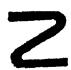
\includegraphics[keepaspectratio]{images/part001_de955d1b.jpg}}

这个命题有重要的推论，将在第九章 § 4 中考察。

第 1 目例 2 中的非豪斯多夫拟紧空间 X 既不满足公理 (O \(_{III}\) )，更不满足命题 2 所述的性质，因为这个空间的任意两个非空开集总相交。

\subsection{拟紧集；紧集；相对紧集}

定义 2. 拓扑空间 X 的子集 A 称为拟紧集（相应地，紧集），如果子空间 A 是拟紧的（相应地，紧的）。

拓扑空间 X 的子集 A 是拟紧集，当且仅当每个由 X 的开集组成的 A 的覆盖都包含 A 的一个有限覆盖；这由公理 (C'\,') 得出。在豪斯多夫空间中，拟紧集与紧集这两个概念相同，因为每个子空间都是豪斯多夫的。

例. 1) 在拓扑空间 X 中，每个有限子集都是拟紧的；空集与每个单点集都是紧的。2) 在拓扑空间 X 中，设 \((x_{n})_{n\in \mathbb{N}}\) 是收敛于一点 \(a\) 的一个无穷点列；则由诸点 \(x_{n}\)（\(n\in \mathbb{N}\)）与 \(a\) 组成的集合 A 是拟紧的。因为若 \((\mathrm{U}_{\iota})\) 是由 X 的开集组成的 A 的一个覆盖，则 \(a\in \mathrm{U}_{\iota}\) 对某个指标 \(\iota\) 成立。\(\mathrm{U}_{\iota}\) 是 \(a\) 的邻域，因此只有有限多个指标 \(n_k\) 使 \(x_{nk}\notin \mathrm{U}_{\iota}\)。对每个指标 \(k\)，设 \(\iota_{k}\) 是使 \(x_{nk}\in \mathrm{U}_{\iota_{k}}\) 的一个指标；则 \(\mathrm{U}_{\iota}\) 与诸 \(\mathrm{U}_{\iota_{k}}\) 构成 A 的一个有限开覆盖。

命题 3. 拟紧（相应地，紧）空间的每个闭子集都是拟紧（相应地，紧）的。

只要注意到：若 A 在 X 中是闭的，则在 A 中闭的每个集合在 X 中也是闭的，这便是公理 (C'') 的直接推论。

命题 4. 豪斯多夫空间的每个紧子集都是闭的。

设 A 是豪斯多夫空间 X 的一个紧子集，并设 x 是 \(\overline{A}\) 的任一点；我们要证明 \(x \in A\)。由假设，x 的每个邻域都与 A 相交，因此 x 在 X 中的邻域滤子 B 在 A 上诱导一个滤子 \(B_{A}\)；A 是紧的，故 \(B_{A}\) 有一个聚点 \(y \in A\)。既然滤子 B 比 \(B_{A}\)（视为 X 上的一个滤子基）在 X 上生成的滤子更粗，y 也是 B 的聚点；于是 y = x，因为 B 在 X 中收敛于 x，且 X 是豪斯多夫的（§ 8，第 1 目，命题 1）。

推论. 在紧空间 X 中，子集 A 是紧的，当且仅当它在 X 中是闭的。

命题 5. 拓扑空间中拟紧子集的一个有限族的并是拟紧的。

只需证明：若 A 与 B 是拓扑空间 X 的两个拟紧子集，则 \(A \cup B\) 是拟紧的。设 R 是 \(A \cup B\) 的一个覆盖；则 R 既是 A 的覆盖又是 B 的覆盖；于是 R 包含 A 的一个有限覆盖 \(R_{1}\) 与 B 的一个有限覆盖 \(R_{2}\)；从而 \(R_{1} \cup R_{2}\) 是 \(A \cup B\) 的一个包含于 R 中的有限覆盖。

定义 3. 拓扑空间 X 的子集 A 称为 X 中相对拟紧（相应地，相对紧）的，如果 A 包含于 X 的一个拟紧（相应地，紧）子集之中。

为简便起见，当关于 X 没有歧义时，我们也说 A 是“相对拟紧集”（相应地，“相对紧集”）。在豪斯多夫空间中，相对拟紧集与相对紧集这两个概念相同。

命题 6. 若 X 是豪斯多夫空间，则 X 的子集 A 是相对紧的，当且仅当 \(\overline{A}\) 是紧的。

若 A 是相对紧的，则由命题 4 及其推论，\(\overline{A}\) 是紧的；反向的蕴含是显而易见的。

命题 7. 若 A 是拓扑空间 X 的一个相对拟紧子集，则 A 上的每个滤子基在 X 中都有一个聚点。

因为若 \(\mathbf{A} \subset \mathbf{K}\)，其中 \(\mathbf{K}\) 是 \(\mathbf{X}\) 的一个拟紧子集，则 \(\mathbf{A}\) 上的每个滤子基在 \(\mathbf{K}\) 中都有一个聚点。

这个命题的逆命题在对 X 不加限制时并不成立（习题 22）。

\pandocbounded{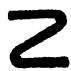
\includegraphics[keepaspectratio]{images/part001_f875b0ae.jpg}}

注. 在非豪斯多夫空间中，紧集未必是闭的，其闭包也未必是拟紧的（习题 5）；两个紧集的交未必是拟紧的（习题 5）；两个紧集的并未必是紧的（习题 5）。

\subsection{紧空间在连续映射下的象}

定理 2. 若 \(f\) 是拟紧空间 \(\mathbf{X}\) 到拓扑空间 \(\mathbf{X}'\) 中的一个连续映射，则集合 \(f(\mathbf{X})\) 是拟紧的。

设 \(\Re\) 是 \(f(\mathbf{X})\) 的一个由 \(\mathbf{X}'\) 中开集组成的覆盖；则 \(\overline{f}^{1}(\Re)\) 是 \(\mathbf{X}\) 的一个开覆盖（\(\S 2\)，第 1 目，定理 1）；于是存在有限子集 \(\mathfrak{S}\)（\(\Re\) 的），使 \((\mathfrak{S}\overline{f}^{1})\) 是 \(\mathbf{X}\) 的一个覆盖；但这时 \(\mathfrak{S}\) 就是 \(f(\mathbf{X})\) 的一个覆盖，定理得证。

推论 1. 设 \(f\) 是拓扑空间 \(\mathbf{X}\) 到豪斯多夫空间 \(\mathbf{X}'\) 中的一个连续映射。则在 \(f\) 之下，\(\mathbf{X}\) 中任一拟紧（相应地，相对拟紧）集的象是 \(\mathbf{X}'\) 中的一个紧（相应地，相对紧）集。

推论 2. 每个连续映射 \(f\)（拟紧空间 \(X\) 到豪斯多夫空间 \(X'\) 中的）都是闭映射。若此外 \(f\) 还是双射，则 \(f\) 是一个同胚。

这由第 3 目的推论 1 与命题 4 立即得出。

特别地：

推论 3. 比拟紧空间的拓扑更粗的豪斯多夫拓扑必与后者一致。

推论 4. 设 X 是一个拓扑空间，R 是 X 上的一个豪斯多夫等价关系。

\begin{enumerate}
\def\labelenumi{\alph{enumi})}
\item
  若 X 中存在一个与每个模 R 等价类都相交的拟紧集 K，则 X/R 是紧的，且 \(K/R_{K}\) 到 X/R 上的典范映射是一个同胚。
\item
  若 K 与每个等价类还只交于一点，则 K 是 X 关于关系 R 的一个连续截面（§ 3，第 5 目）。
\end{enumerate}

设 \(f\) 是限制到 \(K\) 上的典范映射 \(X \to X / R\)。既然 \(X / R\) 是豪斯多夫的，由推论 1 得出 \(X / R\) 是紧的；又由推论 2 得出 \(f\) 是闭映射；于是双射 \(K / R_K \to X / R\)（伴随于 \(f\)）是一个同胚（§ 5，第 2 目，命题 3）。这就处理了 a)；b) 立即得出，因为这时有 \(K / R_K = K\)。

\subsection{紧空间的积}

定理 3（Tychonoff）. 拟紧（相应地，紧）空间的每个积都是拟紧（相应地，紧）的。反之，若非空空间的积是拟紧（相应地，紧）的，则每个因子都是拟紧（相应地，紧）的。

鉴于 § 8 第 2 目命题 7 给出的豪斯多夫积空间的刻画，只需对拟紧空间证明这些断言。若 \(\mathbf{X} = \prod_{\iota \in I} \mathbf{X}_{\iota}\) 是拟紧的且非空，则由第 4 目定理 2，\(\mathbf{X}_{\iota}=\mathrm{pr}_{\iota}(\mathbf{X})\) 是拟紧的。反之，设诸 \(X_{\iota}\) 是拟紧的，并设 U 是 X 上的一个超滤子；则对每个 \(\iota\in I\)，\(\mathrm{pr}_{\iota}(\mathfrak{U})\) 是 \(X_{\iota}\) 上的一个超滤子基（§ 6，第 6 目，命题 10），由公理 (C') 它收敛；于是 U 收敛（§ 7，第 6 目，命题 10 的推论 1），因此 X 是拟紧的。

推论. 拓扑空间之积的一个子集是相对拟紧的，必要且充分的是，它的每个投影在相应的因子中都是相对拟紧的。

必要性由 § 4 定理 2 得出。为证充分性，设 A 是 \(\prod_{i} X_{i}\) 的一个子集，使得对每个指标 \(i\)，\(\operatorname{pr}_{i}(A)\) 包含于拟紧子集 \(K_{i}\)（\(X_{i}\) 的）中；则 A 包含于拟紧子集 \(\prod_{i} K_{i}\)（\(\prod_{i} X_{i}\) 的）中。

\subsection{紧空间的逆极限}

命题 8. 设 \((\mathbf{X}_{\alpha}, f_{\alpha \beta})\) 是由有向集 I 加标的紧空间的一个逆系统，使得 \(f_{\alpha \alpha}\) 对每个 \(\alpha \in \mathbf{I}\) 是恒同映射。设 \(\mathbf{X} = \varprojlim \mathbf{X}_{\alpha}\) 是逆极限，\(f_{\alpha}: \mathbf{X} \to \mathbf{X}_{\alpha}\) 是典范映射（§ 4，第 4 目）。则

\begin{enumerate}
\def\labelenumi{\alph{enumi})}
\tightlist
\item
  X 是紧的，且对每个 \(\alpha \in I\) 我们有
\end{enumerate}

\[
f _ {\alpha} (\mathbf {X}) = \bigcap_ {\beta \geqslant \alpha} f _ {\alpha \beta} (\mathbf {X} _ {\beta}).\tag{I}
\]

\begin{enumerate}
\def\labelenumi{\alph{enumi})}
\setcounter{enumi}{1}
\tightlist
\item
  若诸 \(\mathbf{X}_{\alpha}\) 都非空，则 \(\mathbf{X}\) 非空。
\end{enumerate}

X 是 \(\prod_{\alpha} X_{\alpha}\) 的一个闭子空间（§ 8，第 2 目，命题 7，推论 2）

而后者由第 5 目定理 3 与第 3 目命题 3 是紧的。其余断言是《集合论》第三章 § 7 第 4 目定理 1 的推论。我们应用这个定理时，取 \(\mathfrak{S}_{\alpha}\) 为 \(\mathbf{X}_{\alpha}\) 的闭子集组成的集合。条件 (i) 与 (ii) 分别就是公理 \((\mathrm{O}_{\mathbf{i}}^{\prime})\) 与 \((\mathbf{C}^{\prime \prime})\)；条件 (iii) 得以满足，因为 \(\{x_{\alpha}\}\) 是闭的且 \(f_{\alpha \beta}\) 连续（\(\S 2\)，第 1 目，定理 1）；最后，条件 (iv) 由第 4 目定理 2 的推论 2 得以满足。

推论 1. 设 \((\mathbf{X}_{\alpha}, f_{\alpha\beta})\) 是由一个有向集加标的拓扑空间的逆系统，使得对每对指标 \(\alpha\), \(\beta\)（满足 \(\alpha \leqslant \beta\)）及每个 \(x_{\alpha} \in X_{\alpha}\)，\(\overline{f}_{\alpha\beta}(x_{\alpha})\) 是紧的。则等式 (1) 成立，且 \(\overline{f}_{\alpha}(x_{\alpha})\) 对每个 \(\alpha\) 与每个 \(x_{\alpha} \in X_{\alpha}\) 是紧的。

对每个 \(x_{\alpha} \in \bigcap_{\beta \geqslant \alpha} f_{\alpha \beta}(X_{\beta})\) 及每个 \(\beta \geqslant \alpha\)，令 \(L_{\beta}\) 表示 \(\overline{f}_{\alpha \beta}^{1}(x_{\alpha})\)。若 \(\alpha \leqslant \beta \leqslant \gamma\)，则我们有 \(f_{\beta \gamma}(L_{\gamma}) \subset L_{\beta}\)，且满足 \(\beta \geqslant \alpha\) 的全体指标组成的集合在指标集中是共尾的。由此立即得出，诸 \(L_{\beta} (\beta \geqslant \alpha)\) 构成拓扑空间的一个逆系统（以诸 \(f_{\beta \gamma}\) 的限制为映射），其逆极限 \(L\) 同胚于 \(\overline{f}_{\alpha}^{1}(x_{\alpha})\)。既然由假设诸 \(L_{\beta}\) 是紧的且非空，该推论由命题 8 得出。

推论 2. 设 \((\mathbf{X}_{\alpha}, f_{\alpha \beta})\) 与 \((\mathbf{X}_{\alpha}^{\prime}, f_{\alpha \beta}^{\prime})\) 是由同一有向集 I 加标的拓扑空间的两个逆系统，并设 \((u_{\alpha})\) 是映射 \(u_{\alpha}: \mathbf{X}_{\alpha} \to \mathbf{X}_{\alpha}^{\prime}\) 的一个逆系统。设 \(\mathbf{X} = \varprojlim \mathbf{X}_{\alpha}\)，\(\mathbf{X}^{\prime} = \varprojlim \mathbf{X}_{\alpha}^{\prime}\)，\(u = \varprojlim u_{\alpha}\)。则：

\begin{enumerate}
\def\labelenumi{\alph{enumi})}
\item
  若 \(x' = (x_{\alpha}') \in \mathbf{X}'\) 使 \(\overline{u}_{\alpha}(x_{\alpha}')\) 对每个 \(\alpha \in I\) 是紧的且非空，则 \(\overline{u}^1(x')\) 是紧的且非空。
\item
  若诸 \(X_{\alpha}\) 是紧的，诸 \(X_{\alpha}^{\prime}\) 是豪斯多夫的，且诸 \(u_{\alpha}\) 是满射与连续的，则 u 是满射。
\end{enumerate}

令 \(\mathbf{L}_{\alpha}\) 表示 \(\overline{\boldsymbol{u}}_{\alpha}^{1}(x_{\alpha}^{\prime})\)；则显然诸 \(\mathbf{L}_{\alpha}\) 构成拓扑空间的一个逆系统（以诸 \(f_{\alpha \beta}\) 的限制为映射），且 \(\overline{\boldsymbol{u}}^{1}(x^{\prime} = \mathbf{L})\) 是诸 \(\mathbf{L}_{\alpha}\) 的逆极限；因此断言 a) 由命题 8 得出。鉴于第 3 目命题 3，断言 b) 是一个直接推论。

\subsection{局部紧空间}

定义 4. 拓扑空间 X 称为局部紧的，如果它是豪斯多夫的且 X 的每一点都有一个紧邻域。

显然紧空间是局部紧的，但反之不真；例如，每个离散空间都是局部紧的，但若是无限的则不是紧的。

* 我们将在第四章 § 2 中看到，实直线 R 是局部紧的，但不是紧的。*

命题 9. 每个局部紧空间都是正则的。

设 X 是局部紧空间，则每点 \(x \in X\) 都有一个紧邻域 V；既然 X 是豪斯多夫的，V 是闭的（第 3 目，命题 4）。另一方面，V 是 X 的正则子空间（第 2 目，命题 1 的推论），因此 X 是正则的（§ 8，第 4 目，命题 13）。

推论. 在局部紧空间中，每一点都有一个紧邻域组成的基本邻域系。

因为 x 的一个闭邻域与 x 的一个紧邻域之交是 x 的一个紧邻域（第 3 目，命题 3）。

\pandocbounded{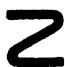
\includegraphics[keepaspectratio]{images/part001_13daf5c9.jpg}}

存在这样的非豪斯多夫拓扑空间，其中每一点都有一个由紧邻域组成的基本邻域系（习题 5）。

命题 9 的推论可以如下推广：

命题 10. 在局部紧空间 X 中，每个紧集 K 都有一个由紧邻域组成的基本邻域系。

设 \(\mathbf{U}\) 是 \(\mathbf{K}\) 的任一邻域。对每个 \(x \in \mathbf{K}\)，存在紧邻域 \(\mathbf{W}(x)\)（即 \(x\) 的紧邻域），它包含于 \(\mathbf{U}\)。当 x 跑遍 K 时，诸集合

W (x) 的内部构成 K 的一个开覆盖；于是存在有限多个点 \(x_{i} \in K\)（\(1 \leqslant i \leqslant n\)），使诸 \(W(x_{i})\) 的内部覆盖 K。因此诸 \(W(x_{i})\) 的并 V 是 K 的一个包含于 U 中的紧邻域（第 3 目，命题 5）。

命题 11. 设 X 是局部紧空间，F 是 X 的一个子集，使得每当 K 是 X 的紧子集时 \(F \cap K\) 都是紧的。则 F 在 X 中是闭的。

鉴于第 3 目命题 4，这由 § 3 第 1 目命题 3 a) 得出。

命题 12. 在豪斯多夫空间 X 中，每个局部紧子空间 A 都是局部闭的。

由假设，对每个 \(x \in A\)，存在 x 在 X 中的一个邻域 V，使得 \(V \cap A\) 是紧的，从而在 V 中是闭的（第 3 目，命题 4）。

命题 13. 局部紧空间 X 的每个局部闭子空间都是局部紧的。

设 A 是 X 的一个局部闭子空间；则对每个 \(x \in A\)，存在 x 在 X 中的一个邻域 U，使得 \(U \cap A\) 在 U 中是闭的。设 \(V \subset U\) 是 x 在 X 中的一个紧邻域；\(V \cap A = V \cap (U \cap A)\) 在 V 中是闭的，从而是紧的（第 3 目，命题 3）。既然 \(V \cap A\) 是 x 在 A 中的一个邻域，结论得证（显然 A 是豪斯多夫的）。

\pandocbounded{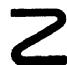
\includegraphics[keepaspectratio]{images/part001_5df2d3a1.jpg}}

定理 1（第 1 目）与定理 2 的推论 2（第 4 目）不能推广到非紧的局部紧空间。

例如，在无限离散空间 X 中，由包含给定点 \(x \in X\) 且余集有限的那些集合组成的滤子以 x 为唯一聚点，但不收敛于 x。既然 X 到豪斯多夫空间 \(X'\) 中的任何映射 f 都连续，f 之下 X 的任一子集（因 X 是离散的，它在 X 中是闭的）的象一般不是 \(X'\) 的闭子集。

与第 5 目定理 3 相应的命题如下：

命题 14. a) 设 \((\mathbf{X}_{\iota})_{\iota \in I}\) 是局部紧空间的一个族，使得除有限多个指标外 \(\mathbf{X}_{\iota}\) 都是紧的。则积空间 \(\mathbf{X} = \prod_{\iota \in I} \mathbf{X}_{\iota}\) 是局部紧的。

\begin{enumerate}
\def\labelenumi{\alph{enumi})}
\setcounter{enumi}{1}
\item
  反之，若非空拓扑空间的族 \((\mathbf{X}_{\iota})_{\iota\in I}\) 的积是局部紧的，则除有限多个指标外诸因子 \(\mathbf{X}_{\iota}\) 都是紧的，且不紧的那些因子是局部紧的。
\item
  设 \(x = (x_{\iota})\) 是 \(X\) 的一点。对每个指标 \(\iota \in I\)，若 \(X_{\iota}\) 局部紧但不紧，则设 \(V_{\iota}\) 是 \(x_{\iota}\) 在 \(X_{\iota}\) 中的一个紧邻域，而对所有其他指标 \(\iota\) 令 \(V_{\iota} = X_{\iota}\)。则 \(\prod_{\iota \in I} V_{\iota}\) 是 \(x\) 在 \(X\) 中的一个紧邻域（第 5 目，定理 3）。又由 § 8 第 2 目命题 7，\(X\) 是豪斯多夫的，从而是局部紧的。
\item
  若 \(X = \prod_{\iota \in I} X_{\iota}\) 是局部紧的且诸 \(X_{\iota}\) 非空，则每个 \(X_{\iota}\) 同胚于 \(X\) 的一个闭子空间（§ 4，第 2 目，命题 4 及 § 4，第 3 目，命题 7 的推论），于是由命题 13 是局部紧的。设 \(a = (a_{\iota})\) 是 \(X\) 的一点，\(V\) 是 \(a\) 的一个紧邻域；既然除有限多个指标外我们有 \(pr_{\iota}V = X_{\iota}\)（§ 4，第 1 目），则由第 4 目定理 2 的推论 1，除有限多个指标外诸 \(X_{\iota}\) 都是紧的。
\end{enumerate}

\subsection{局部紧空间在紧空间中的嵌入}

定理 4（Alexandroff）. 若 X 是任一局部紧空间，则存在一个紧空间 \(X'\) 以及 X 到 \(X'\) 中一点的余集上的一个同胚 f。此外，设 \(X_{1}'\) 是另一个紧空间，且存在一个同胚 \(f_{1}\) 把 X 映到 \(X_{1}'\) 中一点的余集上，则存在 \(X'\) 到 \(X_{1}'\) 上的唯一一个同胚 g，使得 \(f_{1}=g\circ f\)。

我们先证明定理的第二个断言。设

\[
f (\mathbf {X}) = \mathbf {X} ^ {\prime} - \left\{\omega \right\} \quad \text { and } \quad f _ {1} (\mathbf {X}) = \mathbf {X} _ {1} ^ {\prime} - \left\{\omega_ {1} \right\}.
\]

若同胚 \(g\) 存在，它必是唯一的，因为按定义有 \(g(x') = f_1(\overline{f}^1 (x'))\)（只要 \(x' \neq \omega\)），从而 \(g(\omega) = \omega_1\)。尚须证明这样定义的双射 \(g: \mathbf{X}' \to \mathbf{X}_1'\) 是双连续的；既然 \(\mathbf{X}'\) 与 \(\mathbf{X}_1'\) 可以互换，我们只需证明 \(g\) 之下点 \(x' \in \mathbf{X}'\) 的一个邻域的象是 \(g(x')\) 在 \(\mathbf{X}_1'\) 中的一个邻域。这由 \(g\) 的定义当 \(x' \neq \omega\) 时是显然的。若 \(x' = \omega\)，设 \(V'\) 是 \(\omega\) 在 \(X'\) 中的一个开邻域；则 \(X' - V' = K\) 在 \(X'\) 中是闭的，从而是紧的（第 3 目，命题 3），且包含于 \(f(X)\)；于是 \(g(K) = f_1(\overline{f}^1 (K))\) 是紧的（第 4 目，定理 2，推论 1）。由此得出 \(g(V') = X_1' - g(K)\) 是 \(\omega_1\) 的一个开邻域（第 3 目，命题 4）。因此 \(g\) 是一个同胚。

为证明定理的第一部分，设 \(X'\) 是这样一个集合：它是 X 与由单点 \(\omega\) 组成的集合之和。我们这样在 \(X'\) 上定义一个拓扑：取 \(X'\) 的开集组成的集合 D 由 X 的所有开集以及所有形如 \((\mathbf{X}-\mathbf{K})\cup\{\omega\}\) 的子集组成，其中 K 是 X 的一个紧子集。既然 X 的紧子集的任意交是紧的（第 3 目，命题 3 与命题 4），且紧集的任意闭子集是紧的（第 3 目，命题 3），由此得出 \(\mathfrak{D}\) 满足公理 \((\mathrm{O_I})\)；又既然 X 的紧子集的任意有限并是紧的（第 3 目，命题 5），\(\mathfrak{D}\) 也满足 \((\mathrm{O_{II}})\)。X 的每个紧子集在 X 中是闭的（第 3 目，命题 4），因此 \(\mathbf{X}'\) 的拓扑在 X 上诱导的拓扑就是 X 上原有的拓扑。于是尚须证明 \(\mathbf{X}'\) 是紧的。首先，\(\mathbf{X}'\) 是豪斯多夫的。因为若 \(x, y\) 是 X 的任意两个不同的点，它们在 X 中分别有不相交的开邻域 V, W，而 V, W 在 \(\mathbf{X}'\) 中是开的；另一方面，每个 \(x \in \mathbf{X}\) 在 X 中有一个紧邻域 K，它也是 \(x\) 在 \(\mathbf{X}'\) 中的邻域，而

\[
(\mathbf {X} - \mathbf {K}) \cup \{\omega \}
\]

是 \(\omega\) 在 \(\mathbf{X}'\) 中的一个邻域，且显然不与 \(\mathbf{K}\) 相交。最后，\(\mathbf{X}'\) 是拟紧的。设 \((\mathbf{U}_{\lambda})_{\lambda \in \mathbf{L}}\) 是 \(\mathbf{X}'\) 的一个开覆盖；则至少对一个指标 \(\mu \in \mathbf{L}\) 有 \(\mathbf{U}_{\mu} = (\mathbf{X} - \mathbf{K}_{\mu}) \cup \{\omega\}\)，其中 \(\mathbf{K}_{\mu}\) 是 \(\mathbf{X}\) 的一个紧子集。于是存在有限子集 \(\mathbf{H}\)（\(\mathbf{L}\) 的），使得诸集合 \(\mathbf{U}_{\lambda}\)（\(\lambda \in \mathbf{H}\)）覆盖 \(\mathbf{K}_{\mu}\)；若 \(\mathbf{J} = \mathbf{H} \cup \{\mu\}\)，则 \((\mathbf{U}_{\lambda})_{\lambda \in \mathbf{J}}\) 是 \(\mathbf{X}'\) 的一个有限开覆盖，证明完毕。

注意，若 X 已经是紧的，则 \(\omega\) 是紧空间 \(X'\) 的一个孤立点；故 \(X'\)（\(\S\) 2，第 4 目，例 3）是空间 X 与空间 \(\{\omega\}\) 的和。

当紧空间 \(X'\) 已如上从局部紧空间 X 添加一个元素 \(\omega\) 而构造出来时，常说 \(\omega\) 是 \(X'\) 的“无穷远点”，并说 \(X'\) 是由 X 添加一个无穷远点而得到的。\(X'\) 也称为局部紧空间 X 的 Alexandroff 紧化或单点紧化。

* 例. 若把 Alexandroff 定理应用于实平面 \(\mathbf{R}^2\)，我们就得到一个紧空间，它同胚于球面 \(\mathbf{S}_2\)，其方程为 \(x_1^2 + x_2^2 + x_3^2 = 1\)（在 \(\mathbf{R}^3\) 中）。这两个空间之间的一个同胚可描述如下：点 \(\omega\)（无穷远点，添加于 \(\mathbf{R}^2\)）映到 \((0, 0, 1) \in \mathbf{S}_2\)，而每个点 \((x_1, x_2)\)（\(\mathbf{R}^2\) 的）映到连接点 \((0, 1, 1)\) 与 \((x_1, x_2, 0)\) 的直线（在 \(\mathbf{R}^3\) 中）与 \(\mathbf{S}_2\) 的另一个交点。这个同胚称为球极投影。

\subsection{局部紧 σ 紧空间}

定义 5. 局部紧空间 X 称为 σ 紧的或无穷远处可数的，如果它是紧子集的一个可数并。

例. 1) 离散空间是 \(\sigma\) 紧的当且仅当它是可数的。*2) 实直线 \(\mathbf{R}\) 是局部紧且 \(\sigma\) 紧的，因为它是诸紧区间 \([-n, +n]\)（\(n \in \mathbb{N}\)）的并。*

\pandocbounded{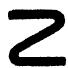
\includegraphics[keepaspectratio]{images/part001_9ca68205.jpg}}

注. 豪斯多夫空间可以是紧子空间的可数并而不是局部紧的。* 例如带弱拓扑的 Hilbert 空间便是如此，我们将在后续卷中证明这一点。

命题 15. 若 X 是局部紧 \(\sigma\) 紧空间，则存在 X 的相对紧开子集的一个序列 \((\mathbf{U}_n)\)，它覆盖 X，且 \(\overline{\mathbf{U}}_n \subset \mathbf{U}_{n+1}\) 对每个 \(n\) 成立。

设 X 是紧集序列 \((\mathbf{K}_{n})\) 的并。设 \(U_{1}\) 是 \(K_{1}\) 的一个相对紧开邻域（第 7 目，命题 10），并归纳地定义 \(U_{n}\)（对 n \textgreater{} 1）为 \(\overline{U}_{n-1} \in K_{n}\) 的一个相对紧开邻域（第 3 目，命题 5；第 7 目，命题 10）。序列 \((\mathbf{U}_{n})\) 显然具有所需的性质。

推论 1. 用命题 15 的记号，X 的每个紧子集 K 都包含于某个 \(U_{n}\) 中。

因为 K 可由有限多个 \(U_{k}\) 覆盖，依据公理 (C'\,')。

推论 2. 设 X 是局部紧空间，X' 是由 X 添加无穷远点 ω 而得到的紧空间（第 8 目）。则 X 是 σ 紧的，当且仅当点 ω 在 X' 中有一个可数的基本邻域系。

若 X 是 σ 紧的，我们可以如命题 15 那样构造 X 的子集序列 \(U_{n}\)，而诸邻域 \(X^{\prime}-\overline{U}_{n}\)（\(\omega\) 在 \(X^{\prime}\) 中的）依据推论 1 构成 \(\omega\) 的一个基本邻域系。反之由如下事实得出：\(\omega\) 的开邻域的余集是 X 的紧子集。

显然，局部紧 \(\sigma\) 紧空间的每个闭子空间都是局部紧且 \(\sigma\) 紧的。同样，局部紧 \(\sigma\) 紧空间的任意有限积是局部紧且 \(\sigma\) 紧的。

但要注意，紧空间的开子空间未必是 \(\sigma\) 紧的，正如 Alexandroff 定理（第 8 目，定理 4）所示。

\subsection{仿紧空间}

定义 6. 拓扑空间称为仿紧的，如果它是豪斯多夫的且满足以下公理：

(PC) X 的每个开覆盖 \(\Re\) 都有一个局部有限开加细 \(\Re'\)。（《集合论》，第二章，§ 4，第 6 目，定义 5）。

显然每个紧空间都是仿紧的。每个离散空间 X 都是仿紧的，因为由 X 的所有单点集组成的开覆盖是局部有限的，且比 X 的每个开覆盖都细。

命题 16. 仿紧空间 X 的每个闭子空间 F 都是仿紧的。

当然 F 是豪斯多夫的。另一方面，若 \((\mathbf{V}_{\iota})\) 是子空间 F 中的一个开覆盖，则每个 \(V_{\iota}\) 形如 \(V_{\iota} = U_{\iota} \cap F\)，其中 \(U_{\iota}\) 在 X 中是开的。考虑由 \(\complement F\) 与诸 \(U_{\iota}\) 组成的 X 的开覆盖 R；既然 X 是仿紧的，R 有一个局部有限加细 \(R'\)，而属于 \(R'\) 的诸集合与 F 的交构成 F 的一个局部有限开覆盖，它比给定的覆盖 \((\mathbf{V}_{\iota})\) 更细。

另一方面，紧空间的开子空间未必是仿紧的（习题 11）。

命题 17. 仿紧空间与紧空间的积是仿紧的。

设 X 是仿紧空间，Y 是紧空间，R 是 \(X \times Y\) 的一个开覆盖。对每个 \((x, y) \in X \times Y\)，存在 x 在 X 中的一个开邻域 \(V(x, y)\) 与 y 在 Y 中的一个开邻域 \(W(x, y)\)，使得 \(V(x, y) \times W(x, y)\) 包含于属于 R 的某个集合中。对每个 \(x \in X\)，当 y 跑遍 Y 时诸集合 \(W(x, y)\) 构成 Y 的一个开覆盖；因此存在有限多个点

\[
y _ {i} \in Y \quad (1 \leqslant i \leqslant n (x))
\]

使得诸 \(\mathbf{W}(x, y_i)\) 覆盖 \(\mathbf{Y}\)。设 \(\mathbf{U}(x)\) 表示

\[
\bigcap_ {i = 1} ^ {n (x)} \mathrm{V} (x, y _ {i});
\]

则诸开集 \(\mathbf{U}(x) \times \mathbf{W}(x, y_i)\) 中的每一个都包含于 \(\Re\) 的某个集合中。现在设 \((\mathbf{T}_{\iota})_{\iota \in \mathbf{I}}\) 是 \(\mathbf{X}\) 的一个局部有限开覆盖，它加细覆盖 \((\mathbf{U}(x))_{x \in \mathbf{X}}\)。对每个 \(\iota \in \mathbf{I}\)，设 \(x_{\iota}\) 是 \(\mathbf{X}\) 中一点，使得 \(\mathbf{T}_{\iota} \subset \mathbf{U}(x_{\iota})\)，并用 \(\mathbf{S}_{\iota,k}\) 表示诸集合 \(\mathbf{W}(x_{\iota}, y_k)\)（它们对应于这个点 \(x_{\iota}\)）（\(1 \leqslant k \leqslant n(x_{\iota})\)）。显然诸集合

\[
\mathrm{T} _ {\iota} \times \mathrm{S} _ {\iota, k} \quad (\iota \in \mathrm{I}, 1 \leqslant k \leqslant n (x _ {\iota}) \text {   for   each   } \iota \in \mathrm{I})
\]

构成 \(\mathbf{X} \times \mathbf{Y}\) 的一个加细 \(\Re\) 的开覆盖，而只要证明这个覆盖是局部有限的，证明即可完成。设 \((x, y)\) 是 \(\mathbf{X} \times \mathbf{Y}\) 的任意一点；存在邻域 \(\mathbf{Q}\)（即 \(x\) 的邻域），它只与有限多个集合 \(\mathbf{T}_{\iota}\) 相交，因而邻域 \(\mathbf{Q} \times \mathbf{Y}\)（\((x, y)\) 的）只与有限多个集合 \(\mathbf{T}_{\iota} \times \mathbf{S}_{\iota,k}\) 相交。

另一方面，两个仿紧空间的积未必是仿紧的（见第九章，§ 5，习题 16）。

命题 18. 仿紧空间族 \((\mathbf{X}_{\iota})_{\iota\in I}\) 的和（§ 2，第 4 目，例 3）是仿紧的。

设 X 是诸 \(X_{\iota}\) 的和，\((\mathrm{V}_{\lambda})_{\lambda\in\mathbf{L}}\) 是 X 的一个开覆盖。由开集 \(X_{\iota}\cap V_{\lambda}\) 组成的覆盖比 \((\mathrm{V}_{\lambda})\) 更细。对每个 \(\iota\in I\)，设 \((\mathrm{U}_{\iota,\mu})_{\mu\in\mathbf{M}_{\iota}}\) 是覆盖 \((\mathrm{V}_{\lambda}\cap\mathrm{X}_{\iota})_{\lambda\in\mathbf{L}}\) 的一个局部有限开加细；则由

\[
\mathbf {U} _ {\iota , \mu} \quad (\iota \in \mathbf {I}, \mu \in \mathbf {M} _ {\iota} \text {   for   each   } \iota \in \mathbf {I})
\]

组成的 X 的开覆盖是局部有限的，且加细原来的覆盖 \((\mathbf{V}_{\lambda})\)。

定理 5. 局部紧空间 X 是仿紧的，当且仅当 X 是局部紧 σ 紧空间族的一个和。

设 X 是仿紧的，并对每个 \(x \in X\) 设 \(V_x\) 是 x 在 X 中的一个相对紧开邻域。则由假设，存在 X 的一个局部有限开覆盖 \((\mathrm{U}(\alpha))_{\alpha \in \Lambda}\)，它加细覆盖 \((\mathrm{V}_x)_{x \in \mathbf{X}}\)。因此诸 \(\mathrm{U}(\alpha)\) 都是相对紧的。X 的每个紧子集 K 只与有限多个集合 \(\mathrm{U}(\alpha)\) 相交，因为非空集合 \(\mathrm{U}(\alpha) \cap \mathrm{K}\) 构成紧空间 X 的一个局部有限开覆盖；故它们必定只有有限个（第 1 目）。现在设 R 是 X 的两点 x, y 之间的如下关系：“存在 A 中的有限指标序列 \((\alpha_i)_{1 \leqslant i \leqslant n}\)，使得 \(x \in \mathrm{U}(\alpha_1)\)，\(y \in \mathrm{U}(\alpha_n)\)，且 \(\mathrm{U}(\alpha_i)\) 与 \(\mathrm{U}(\alpha_{i+1})\)（对 \(1 \leqslant i \leqslant n - 1\)）相交”。立即可以验证 R 是一个等价关系，且每个模 R 等价类都是 X 的开子集{[}因为诸 \(\mathrm{U}(\alpha)\) 是开集{]}。因此 X 是由模 R 的诸等价类构成的局部紧子空间（第 7 目，命题 13）的和，剩下只需证明这些子空间中的每一个都是族 \((\mathrm{U}(\alpha))\) 的一个可数子族之并。

设 \(x\) 是 \(\mathbf{X}\) 的任意一点，定义相对紧开子集的一个序列 \((\mathbf{C}_n)\)（\(\mathbf{X}\) 中的；对 \(n\) 用归纳法）如下：\(\mathbf{C}_1\) 是诸集合 \(\mathbf{U}(\alpha)\)（包含 \(x\) 的）之并，而对每个 \(n > 1\)，\(\mathbf{C}_n\) 是诸集合 \(\mathbf{U}(\alpha)\)（与 \(\mathbf{C}_{n-1}\) 相交的）之并。对 \(n\) 用归纳法立即可以验证，每个 \(\mathbf{C}_n\) 都是相对紧的，且是有限多个集合 \(\mathbf{U}(\alpha)\) 之并。此外，\(x\) 关于 \(\mathbf{R}\) 的等价类是诸 \(\mathbf{C}_n\) 之并：因为若 \((\alpha_i)_{1 \leqslant i \leqslant n}\) 是一个指标序列，使得 \(x \in \mathbf{U}(\alpha_1)\)，且 \(\mathbf{U}(\alpha_i)\) 与 \(\mathbf{U}(\alpha_{i+1})\)（对 \(1 \leqslant i \leqslant n - 1\)）相交，则对 \(i\) 用归纳法可以看出，\(\mathbf{U}(\alpha_i) \subset \mathbf{C}_i\)（对 \(1 \leqslant i \leqslant n\)）。由此推出模 \(\mathbf{R}\) 的诸等价类都是 \(\sigma\) 紧的，这就完成了定理第一部分的证明。

为证其逆，我们可以假设（由命题 18）X 是 σ 紧的。设 \(\Re = (G_{\lambda})_{\lambda \in L}\) 是 X 的任意一个开覆盖，\((U_n)\) 是 X 中具有第 9 目命题 15 所述性质的相对紧开集序列。设 \(K_n\) 表示紧集 \(\overline{U}_n - U_{n-1}(U_n = \emptyset\)，若 \(n \leqslant 0)\)。由构造，开集 \(U_{n+1} - \overline{U}_{n-2}\) 是 \(K_n\) 的一个邻域；因此对每个 \(x \in K_n\)，存在邻域 \(W_x\)（即 \(x\) 的邻域），它包含于某个集合 \(G_{\lambda}\) 中，且也包含于 \(U_{n+1} - \overline{U}_{n-2}\) 中。既然 \(K_n\) 是紧的，有限多个集合 \(W_x\) 便覆盖 \(K_n\)；设 \(H_{ni}(1 \leqslant i \leqslant p_n)\) 是这些集合。于是族 \(\Re'\)（由诸集合 \(H_{ni}(n \geqslant 1, 1 \leqslant i \leqslant p_n\)，对每个 \(n\)) 组成）是 X 的一个加细 \(\Re\) 的开覆盖，因此为完成证明，只须证明 \(\Re'\) 是局部有限的。设 \(z\) 是 X 的任意一点，\(n\) 是使 \(z \in U_n\) 的最小整数；则由于 \(z \notin U_{n-1}\)，存在 \(z\) 的一个邻域 T，它包含于 \(U_n\) 中且不与 \(U_{n-2}\) 相交。由此推出 T 只与那些集合 \(H_{mi}\)（对它们 \(n - 2 \leqslant m \leqslant n + 1\)）相交，即 T 只与 \(\Re'\) 的有限多个集合相交。

在证明过程中我们还建立了如下结果：

推论. 设 X 是局部紧仿紧空间。则 X 的每个开覆盖 R 都有一个由相对紧集组成的局部有限开加细 R'。若 X 是 σ 紧的，则可取 R' 为可数的。

\section{逆紧映射}

在本节中，我们用 \(\iota_{\mathbf{X}}\) 表示集合 \(\mathbf{X}\) 到其自身的恒等映射。

\subsection{逆紧映射}

若 \(f: \mathbf{X} \to \mathbf{Y}\) 与 \(f': \mathbf{X}' \to \mathbf{Y}'\) 是两个连续闭映射，则积 \(f \times f': \mathbf{X} \times \mathbf{X}' \to \mathbf{Y} \times \mathbf{Y}'\) 未必是闭映射，即使 \(f\) 形如 \(\iota_{\mathbf{X}}\)。

例. 到豪斯多夫空间中的每个常值映射都是闭的。但若 \(f\) 是常值映射 \(\mathbf{Q} \to 0\)，则 \(f \times \iota_{\mathbf{Q}}\) 是映射 \((x, y) \to (0, y)\)（\(\mathbf{Q}^2\) 到 \(\mathbf{Q}^2\) 中的），即第二个投影，它不是闭的（§ 4，第 2 目，注 1）。

定义 1. 设 \(f\) 是拓扑空间 \(\mathbf{X}\) 到拓扑空间 \(\mathbf{Y}\) 中的一个映射。称 \(f\) 是逆紧的，如果 \(f\) 是连续的，并且映射 \(f \times \iota_{\mathbf{Z}} : \mathbf{X} \times \mathbf{Z} \to \mathbf{Y} \times \mathbf{Z}\) 对每个拓扑空间 \(\mathbf{Z}\) 都是闭的。

我们将在第 2 目与第 3 目中给出逆紧映射的其他刻画。

如果在定义 1 中取空间 Z 由一个点组成，便得到：

命题 1. 每个逆紧映射都是闭的。

命题 2. 设 \(f: \mathbf{X} \to \mathbf{Y}\) 是一个连续单射。则以下三个命题等价：

\begin{enumerate}
\def\labelenumi{\alph{enumi})}
\item
  \(f\) 是逆紧的。
\item
  \(f\) 是闭的。
\item
  \(f\) 是 \(\mathbf{X}\) 到 \(\mathbf{Y}\) 的一个闭子集上的一个同胚。
\end{enumerate}

我们刚才已见 a) 蕴含 b)。由于等价关系 \(f(x) = f(x')\) 就是相等关系，X 关于这个关系的商空间可与 X 等同；故由 § 5，第 2 目，命题 3，b) 蕴含 c)。最后，若 c) 成立，则 \(f \times \iota_{\mathbf{Z}}\) 是 \(\mathbf{X} \times \mathbf{Z}\) 到 \(\mathbf{Y} \times \mathbf{Z}\) 的一个闭子空间上的一个同胚，因而是闭映射；故 c) 蕴含 a)。

命题 3. 设 \(f: \mathbf{X} \to \mathbf{Y}\) 是一个连续映射。若 \(\mathbf{T}\) 是 \(\mathbf{Y}\) 的任意子集，用 \(f_{\mathbf{T}}\) 表示映射 \(\overline{f}^{1}(\mathbf{T}) \to \mathbf{T}\)，它与 \(f\) 在 \(\overline{f}^{1}(\mathbf{T})\) 上取值相同。

\begin{enumerate}
\def\labelenumi{\alph{enumi})}
\item
  若 \(f\) 逆紧，则 \(f_{\mathbf{T}}\) 也逆紧。
\item
  设 \((\mathrm{T}(\iota))_{\iota\in I}\) 是 Y 的一个子集族，其诸内部覆盖 Y，或者它是 Y 的一个局部有限闭覆盖；则若诸映射 \(f_{\mathbf{T}(\iota)}\) 都逆紧，\(f\) 也逆紧。
\end{enumerate}

设 \(\mathbf{Z}\) 是一个拓扑空间。若 \(\mathbf{T}\) 是 \(\mathbf{Y}\) 的任意子集，我们有

\[
f _ {\mathbf {T}} \times \iota_ {\mathbf {Z}} = (f \times \iota_ {\mathbf {Z}}) _ {\mathbf {T} \times \mathbf {Z}};
\]

若 \(f\) 逆紧，则 \(f \times \iota_{\mathbf{Z}}\) 是闭的，因而 \((f \times \iota_{\mathbf{Z}})_{\mathbf{T} \times \mathbf{Z}}\) 也是闭的{[}§ 5，第 1 目，命题 2 a){]}，于是 a) 得证。现在若 \((\mathrm{T}(\iota))_{\iota \in \mathbf{I}}\) 满足 b) 中所述两个条件之一，则覆盖 \((\mathrm{T}(\iota) \times \mathbf{Z})_{\iota \in \mathbf{I}}\)（\(\mathbf{Y} \times \mathbf{Z}\) 的）具有同样的性质；若诸 \(f_{\mathbf{T}(\iota)}\) 逆紧，则诸映射

\[
(f \times \iota_ {\mathbf {Z}}) _ {\mathbf {T} (\iota) \times \mathbf {Z}}
\]

都是闭的，于是 \(f \times \iota_{\mathbf{Z}}\) 是闭的{[}§ 5，第 1 目，命题 2 b){]}。证明完毕。

命题 4. 设 I 是有限集，且对每个 \(i \in I\)，设 \(f_i: X_i \to Y_i\) 是一个连续映射。设 \(X = \prod_{i \in I} X_i\)，\(Y = \prod_{i \in I} Y_i\)，并设 \(f: X \to Y\)

是积映射 \((x_{i})\to (f_{i}(x_{i}))\)。则：

\begin{enumerate}
\def\labelenumi{\alph{enumi})}
\item
  若每个 \(f_i\) 都逆紧，则 \(f\) 逆紧。
\item
  若 \(f\) 逆紧且诸 \(X_i\) 非空，则每个 \(f_i\) 都逆紧。
\end{enumerate}

（我们将在第 2 目，定理 1，推论 3 中看到，这个命题可以推广到无穷积。）

用归纳法，只需考虑 \(\mathbf{I} = \{\mathbf{1},\mathbf{2}\}\) 的情形。a) 设 \(f_{1}, f_{2}\) 逆紧，并设 \(\mathbf{Z}\) 是一个拓扑空间；\(f_{1} \times f_{2} \times \iota_{\mathbf{Z}}\) 是 \(\iota_{\mathbf{Y}_1} \times f_2 \times \iota_{\mathbf{Z}}\) 与

\[
f _ {1} \times \iota_ {\mathbf {X} _ {2}} \times \iota_ {\mathbf {Z}};
\]

的复合；由假设这两个映射都是闭的，故 \(f_{1} \times f_{2} \times \iota_{\mathbf{Z}}\) 也是闭的{[}§ 5，第 1 目，命题 1 a){]}，于是 \(f_{1} \times f_{2}\) 逆紧。

\begin{enumerate}
\def\labelenumi{\alph{enumi})}
\setcounter{enumi}{1}
\tightlist
\item
  现在设 \(f\) 逆紧。设 \(\mathbf{F}\) 是 \(\mathbf{X}_2 \times \mathbf{Z}\) 的一个闭子集，\(\mathbf{G}\) 是 \(\mathbf{F}\) 在 \(\mathbf{Y}_2 \times \mathbf{Z}\) 中（在映射 \(f_2 \times \iota_{\mathbf{Z}}\) 下）的象。则 \(\mathbf{X}_1 \times \mathbf{F}\) 在 \(\mathbf{Y}_1 \times \mathbf{Y}_2 \times \mathbf{Z}\) 中（在 \(f_1 \times f_2 \times \iota_{\mathbf{Z}}\) 下）的象是 \(f_1(\mathbf{X}_1) \times \mathbf{G}\)。由假设，它在 \(\mathbf{Y}_1 \times \mathbf{Y}_2 \times \mathbf{Z}\) 中是闭的；若 \(\mathbf{X}_1 \neq \emptyset\)，则 \(f_1(\mathbf{X}_1)\) 非空，这蕴含 \(\mathbf{G}\) 在 \(\mathbf{Y}_2 \times \mathbf{Z}\) 中是闭的（§ 4，第 3 目，命题 7 的推论）；故 \(f_2\) 逆紧。类似地，\(f_1\) 在 \(\mathbf{X}_2 \neq \emptyset\) 时逆紧。
\end{enumerate}

命题 5. 设 \(f: \mathbf{X} \to \mathbf{X}'\) 与 \(g: \mathbf{X}' \to \mathbf{X}''\) 是两个连续映射。

\begin{enumerate}
\def\labelenumi{\alph{enumi})}
\item
  若 \(f\) 与 \(g\) 都逆紧，则 \(g \circ f\) 逆紧。
\item
  若 \(g \circ f\) 逆紧且 \(f\) 是满射，则 \(g\) 逆紧。
\item
  若 \(g \circ f\) 逆紧且 \(g\) 是单射，则 \(f\) 逆紧。
\item
  若 \(g \circ f\) 逆紧且 \(X'\) 是豪斯多夫的，则 \(f\) 逆紧。
\end{enumerate}

设 \(\mathbf{Z}\) 是一个拓扑空间。我们有

\[
(g \circ f) \times \iota_ {\mathbf {Z}} = (g \times \iota_ {\mathbf {Z}}) \circ (f \times \iota_ {\mathbf {Z}});
\]

若 \(f\) 与 \(g\) 逆紧，则 \(f \times \iota_{\mathbf{Z}}\) 与 \(g \times \iota_{\mathbf{Z}}\) 都是闭的；故{[}§ 5，第 1 目，命题 1 a){]} ( \(g \circ f\) ) × \(\iota_{\mathbf{Z}}\) 是闭的；这就证明了 a)。b){[}相应地，c){]}的证明沿着同样的思路进行，利用 § 5 第 1 目命题 1 的 b){[}相应地，c){]}，并注意到若 \(f\) 是满射（相应地，若 \(g\) 是单射），则 \(f \times \iota_{\mathbf{Z}}\) 是满射（相应地，\(g \times \iota_{\mathbf{Z}}\) 是单射）。最后，为证 d)，考虑交换图

\[
\mathbf {X} \stackrel {\varphi} {\rightarrow} \mathbf {X} \times \mathbf {X} ^ {\prime}\tag{1}
\]

\[
\begin{array}{c} f \downarrow \\ \mathbf {X} ^ {\prime} \xrightarrow [ \psi ]{} \mathbf {X} ^ {\prime \prime} \end{array} \begin{array}{c} \downarrow (g \circ f) \times \iota_ {\mathbf {x} ^ {\prime}} \\ \times \mathbf {X} ^ {\prime} \end{array}
\]

其中 \(\varphi(x) = (x, f(x))\)，\(\psi(x') = (g(x'), x')\)。映射 \(\varphi\)（相应地，\(\psi\)）是 X（相应地，X'）到 \(f\) 的图象（相应地，\(g\) 的图象的镜象）上的一个同胚（\(\S 4\)，第 1 目，命题 1，推论 2）。此外，由于 X' 是豪斯多夫的，图象 \(\varphi(X)\)（即 \(f\) 的图象）在 X × X' 中是闭的（\(\S 8\)，第 1 目，命题 2，推论 2）。故（命题 2）\(\varphi\) 是逆紧的；另一方面，命题 4 表明 ( \(g \circ f\) ) × \(\iota_{X'}\) 是逆紧的。由上面的 a) 及图 (1) 的交换性，\(\psi \circ f\) 是逆紧的；但 \(\psi\) 是单射，故由上面的 c)，\(f\) 是逆紧的。

注. 若 \(\mathbf{X}'\) 不是豪斯多夫的，则可能 \(g \circ f\) 逆紧而 \(f\) 不逆紧；例如，取 \(\mathbf{X}\) 与 \(\mathbf{X}''\) 各由一点组成，\(\mathbf{X}'\) 由两点组成并带最粗拓扑。

推论 1. 若 \(f: \mathbf{X} \to \mathbf{Y}\) 是逆紧映射，则 \(f\) 在闭子集 \(\mathbf{F}\)（\(\mathbf{X}\) 的）上的限制是 \(\mathbf{F}\) 到 \(\mathbf{Y}\) 中的一个逆紧映射。

因为这个限制是复合 \(f \circ j\)，其中 \(j: \mathbf{F} \to \mathbf{X}\) 是典范单射，由命题 2 它是逆紧的。

推论 2. 设 \(f: \mathbf{X} \to \mathbf{Y}\) 是逆紧映射，其中 \(\mathbf{X}\) 是豪斯多夫的。则子空间 \(f(\mathbf{X})\)（\(\mathbf{Y}\) 的）是豪斯多夫的。

由命题 5 c)，只需考虑 \(f(\mathbf{X}) = \mathbf{Y}\) 的情形。此时 \(\mathbf{Y} \times \mathbf{Y}\) 的对角线是 \(f \times f\) 下 \(\mathbf{X}\) 的对角线的象，后者是闭的（§ 8，第 1 目，命题 1）；\(f \times f\) 是逆紧的（命题 4）；故 \(\mathbf{Y} \times \mathbf{Y}\) 的对角线是闭的（命题 1），因此 \(\mathbf{Y}\) 是豪斯多夫的（§ 8，第 1 目，命题 1）。

推论 3. 设 I 是有限集，且对每个 \(i \in I\)，设 \(f_i: X \to Y_i\) 是逆紧映射。若 X 是豪斯多夫的，则映射 \(x \to (f_i(x))\)（X 到 \(\prod_{i \in I} Y_i\) 中的）是逆紧的。

这个映射是积映射 \((x_{i})\to (f_{i}(x_{i}))\)（\(\mathbf{X}^{\mathbf{I}}\) 到 \(\prod_{i}\mathbf{Y}_{i}\) 中的）与 \(\mathbf{X}\) 到 \(\mathbf{X}^{\mathbf{I}}\) 中的对角映射的复合；由于后者是逆紧的（由命题 2 及 § 8，第 1 目，命题 1），结论由命题 4 与命题 5 a) 得出。

推论 4. 设 X 与 Y 是两个拓扑空间，\(f: \mathbf{X} \to \mathbf{Y}\) 是一个连续映射，R 是 X 上的等价关系 \(f(x) = f(y)\)，而

\[
\mathbf {X} \xrightarrow {p} \mathbf {X} / \mathbf {R} \xrightarrow {h} f (\mathbf {X}) \xrightarrow {i} \mathbf {Y}
\]

是 \(f\) 的典范分解。则 \(f\) 逆紧当且仅当 \(p\) 逆紧、\(h\) 是一个同胚且 \(f(\mathbf{X})\) 是 \(\mathbf{Y}\) 的一个闭子集。

由命题 5 a) 与命题 2，这些条件是充分的。反之，若 \(f\) 逆紧，则 \(f\) 是闭的；故 \(f(\mathbf{X})\) 在 \(\mathbf{Y}\) 中是闭的，且 \(h\) 是一个同胚（§ 5，第 2 目，命题 3）；又由命题 5 c)，\(h \circ p\) 是逆紧的；故由命题 5 a)，\(p = \overline{h} \circ (h \circ p)\) 是逆紧的。

\subsection{用紧性刻画逆紧映射}

在本小节中，我们用 P 表示由单独一点组成且带其唯一拓扑的空间。

引理 1. 设 X 是一个拓扑空间，使得常值映射 \(X \rightarrow P\) 是逆紧的。则 X 是拟紧的。

（稍后（定理 1，推论 1）我们将看到这个性质刻画了拟紧空间。）

我们可以限于 X 非空的情形。设 F 是 X 上的一个滤子，\(X' = X \cup \{\omega\}\) 是与 F 相伴的拓扑空间（§ 6，第 5 目，例）。设 \(\Delta\) 是 \(X \times X'\) 的由所有 \((x, x)\)（其中 \(x \in X\)）组成的子集，并设 \(F = \overline{\Delta}\) 是 \(\Delta\) 在 \(X \times X'\) 中的闭包。鉴于关于 X 的假设，F 在投影 \(X \times X' \to X'\) 下的象在 \(X'\) 中是闭的；这个象包含 X，因此包含 \(\omega\)，后者属于 X 的闭包；换言之，存在一点 \(x \in X\)，使得 \((x, \omega) \in F\)。由 \(X \times X'\) 的拓扑的定义，这意味着对 x 在 X 中的每个邻域 V 及每个 \(M \in F\)，有 \((V \times M) \cap \Delta \neq \emptyset\)，即 \(V \cap M \neq \emptyset\)，故 x 是滤子 F 的一个聚点，因此 X 是拟紧的。

证毕。

定理 I. 设 \(f: \mathbf{X} \to \mathbf{Y}\) 是一个连续映射。则以下四个命题等价：

\begin{enumerate}
\def\labelenumi{\alph{enumi})}
\item
  \(f\) 是逆紧的。
\item
  \(f\) 是闭的，且 \(\overline{f}^1(y)\) 对每个 \(y \in \mathbf{Y}\) 都是拟紧的。
\item
  若 \(\mathfrak{F}\) 是 \(\mathbf{X}\) 上的一个滤子，且 \(y\in \mathbf{Y}\) 是 \(f(\mathfrak{F})\) 的一个聚点，则存在一个聚点 \(x\)（\(\mathfrak{F}\) 的），使得 \(f(x) = y\)。
\item
  若 \(\mathfrak{U}\) 是 \(\mathbf{X}\) 上的一个超滤子，且 \(y\in \mathbf{Y}\) 是超滤子基 \(f(\mathfrak{U})\) 的一个极限点，则存在一个极限点 \(x\)（\(\mathfrak{U}\) 的），使得 \(f(x) = y\)。
\item
  \(\Longrightarrow\) b)：若 \(f\) 逆紧，则 \(f\) 是闭的（第 1 目，命题 1），且对每个 \(y \in Y\)，映射 \(f_{\{y\}}: \overline{f}^1(y) \to \{y\}\) 是逆紧的{[}第 1 目，命题 3a){]}。由引理 1，这蕴含 \(\overline{f}^1(y)\) 是拟紧的。
\item
  \(\Longrightarrow\) c)：设 \(\mathfrak{F}\) 与 \(y\) 满足 c) 的假设。设 \(\mathfrak{B}\) 是由 \(\mathfrak{F}\) 的诸集合的闭包组成的 X 上的滤子基。由于 \(f\) 是闭的，我们有 \(f(\overline{\mathbf{M}}) = \overline{f}(\mathbf{M})\)（对每个 \(\mathbf{M} \in \mathfrak{F}\)；§ 5，第 4 目，命题 9）。这表明诸集合 \(\overline{\mathbf{M}} \cap \overline{f}^1(y)\)（\(\mathbf{M} \in \mathfrak{F}\)）都非空，因而构成 \(\overline{f}^1(y)\) 上的一个滤子基，其元素是 \(\overline{f}^1(y)\) 的闭子集。既然 \(\overline{f}^1(y)\) 是拟紧的，存在一点 \(x \in \overline{f}^1(y)\)，它属于所有的集合 \(\overline{\mathbf{M}}\)（当 M 跑遍 \(\mathfrak{F}\) 时）。于是 \(f(x) = y\)，且 \(x\) 是 \(\mathfrak{F}\) 的一个聚点。
\end{enumerate}

\begin{enumerate}
\def\labelenumi{\alph{enumi})}
\setcounter{enumi}{2}
\tightlist
\item
  \(\Longrightarrow\) d)：平凡。
\end{enumerate}

\begin{enumerate}
\def\labelenumi{\alph{enumi})}
\setcounter{enumi}{3}
\tightlist
\item
  \(\Longrightarrow\) a)：我们先证明若 d) 成立，则 \(f\) 是闭映射。设 A 是 X 的一个非空闭子集，\(\mathfrak{F}\) 是 X 的包含 A 的子集组成的滤子。则 A 是 \(\mathfrak{F}\) 的聚点集。设 B 是滤子基 \(f(\mathfrak{F})\) 在 Y 上的聚点集；B 是闭的且显然包含 \(f(A)\)；我们将证明 \(B = f(A)\)。设 \(y \in B\)，\(\mathfrak{B}\) 是 \(y\) 在 Y 中的邻域滤子；则由假设，\(\mathfrak{W} = \overline{f}^{1}(\mathfrak{V})\) 的每个集合都与 \(\mathfrak{F}\) 的每个集合相交；故 \(\mathfrak{W}\) 是 X 上的一个滤子基，且存在 X 上的一个超滤子 \(\mathfrak{U}\)，它比 \(\mathfrak{F}\) 与以 \(\mathfrak{W}\) 为基的滤子都细（§ 6，第 2 目，命题 1，推论 1 及第 4 目，定理 1）。以 \(f(\mathfrak{U})\) 为基的超滤子比 \(\mathfrak{V}\) 细，因此收敛于 \(y\)。依据 d)，存在一点 \(x \in X\)，使得 \(f(x) = y\) 且 \(\mathfrak{U}\) 收敛于 \(x\)；由于 \(\mathfrak{U}\) 比 \(\mathfrak{F}\) 细，\(x\) 是 \(\mathfrak{F}\) 的一个聚点；故 \(x \in A\)。这表明 \(B = f(A)\)，因而 \(f\) 是闭的。
\end{enumerate}

为完成证明，还须证明 \(f \times \iota_{\mathbf{Z}}\) 对每个拓扑空间 \(\mathbf{Z}\) 都是闭的。由已证的结果，只须证明若 \(f\) 满足条件 d)，则 \(f \times \iota_{\mathbf{Z}}\) 也满足。这是下述一般引理的推论：

引理 2. 若 \((f_{\iota})_{\iota\in I}\) 是一族连续映射 \(f_{\iota}:\mathbf{X}_{\iota}\to \mathbf{Y}_{\iota}\)，其中每个都满足定理 1 的条件 d)，则积映射

\[
f: (x _ {\iota}) \rightarrow (f _ {\iota} (x _ {\iota}))
\]

也满足 d)。

设 \(\mathfrak{U}\) 是 \(\mathbf{X} = \prod_{\iota} \mathbf{X}_{\iota}\) 上的一个超滤子，\(y = (y_{\iota})\) 是 \(\mathbf{Y} = \prod_{\iota} \mathbf{Y}_{\iota}\) 的一点，使得 \(f(\mathfrak{U})\) 收敛于 \(y\)。这意味着诸超滤子基 \(\operatorname{pr}_{\iota}(f(\mathfrak{U})) = f_{\iota} (\operatorname{pr}_{\iota}(\mathfrak{U}))\) 中的每一个都收敛于 \(y_{\iota}\)（\(\S 7\)，第 6 目，命题 10，推论 1）。依据条件 d)，对每个 \(\iota \in I\)，存在 \(x_{\iota} \in \mathbf{X}_{\iota}\)，使得 \(f_{\iota}(x_{\iota}) = y_{\iota}\) 且 \(\operatorname{pr}_{\iota}(\mathfrak{U})\) 收敛于 \(x_{\iota}\)；但这样 \(\mathfrak{U}\) 便收敛于 \(x = (x_{\iota})\)（同上），且我们有 \(f(x) = y\)。这就完成了引理 2 从而定理 1 的证明。

推论 1. 拓扑空间 X 是拟紧的，当且仅当映射 \(X \rightarrow P\) 是逆紧的。

把 a) \(\Longleftrightarrow\) b) 应用于 \(\mathbf{X} \to \mathbf{P}\) 即可。

推论 2. 拟紧空间 X 到豪斯多夫空间 Y 中的每个连续映射 f 都是逆紧的。

复合 \(X \xrightarrow{f} Y \to P\) 由推论 1 是逆紧的；故由第 1 目命题 5 d)，f 是逆紧的。或者，利用 § 9，第 4 目，定理 2，推论 2，应用定理 1 的判别准则 b)。

推论 3. 若 \((f_{\iota})\) 是一族逆紧映射，则积映射 \((x_{\iota})\to (f_{\iota}(x_{\iota}))\) 是逆紧的。

鉴于定理 1，这就是上面的引理 2。

若把这个推论应用于映射族 \(X_{\iota} \rightarrow P\) 并利用推论 1，便得到 Tychonoff 定理（§ 9，第 5 目，定理 3）。

推论 4. 设 X 是豪斯多夫空间，\(f_{\iota}: \mathbf{X} \to \mathbf{Y}_{\iota}\) 是一族逆紧映射。则映射 \(f: x \to (f_{\iota}(x))\)（X 到 \(\prod_{\iota} Y_{\iota}\) 中的）是逆紧的。

证明与有限族情形（第 1 目，命题 5，推论 3）相同，利用上面的推论 3 以及 \(\mathbf{X}^{\mathbf{I}}\) 的对角线是闭的这一事实（\(\S\) 8，第 1 目，命题 1）。

推论 5. 若 X 是任意拟紧空间，Y 是任意拓扑空间，则投影 \(\mathbf{pr}_2: \mathbf{X} \times \mathbf{Y} \to \mathbf{Y}\) 是逆紧的。

因为我们可以把 Y 与 \(P \times Y\) 等同，把 \(pr_{2}\) 与 \(X \rightarrow P\) 和 \(\iota_{Y}\) 的积等同，而这两者都是逆紧映射。

例. 设 X 是一个集合，\(f: \mathbf{X} \to \mathbf{X}'\) 是 X 到拓扑空间 \(\mathbf{X}'\) 上的一个映射；用 \(f\) 下 \(\mathbf{X}'\) 的拓扑的逆像来拓扑化 X。则 \(f\) 是逆紧的，因为 \(f\) 是闭的（\(\S 5\)，第 1 目，例 3），且 \(\mathbf{X}'\) 的一个点的逆像是 X 的一个子空间，其拓扑是最粗拓扑，因而是拟紧的。

注. 当 Y 是豪斯多夫空间时，定理 1 的条件 d) 等价于下述条件：

d′) 若 \(\mathfrak{U}\) 是 \(\mathbf{X}\) 上的一个超滤子，使得 \(f(\mathfrak{U})\) 是收敛滤子基，则 \(\mathfrak{U}\) 收敛。

因为若 \(\mathfrak{U}\) 收敛于 \(x\) 且 \(f(\mathfrak{U})\) 收敛于 \(y\)，则 \(\mathbf{Y}\) 中极限的唯一性与 \(f\) 的连续性表明必有 \(y = f(x)\)。同样，当 Y 是豪斯多夫空间时，定理 1 的条件 c) 等价于：

c′) 若 \(\mathfrak{F}\) 是 \(\mathbf{X}\) 上的一个滤子，使得 \(f(\mathfrak{F})\) 有一个聚点，则 \(\mathfrak{F}\) 有一个聚点。

\[
\text { For } \quad \mathrm{c}) \Longrightarrow \mathrm{c} ^ {\prime}) \Longrightarrow \mathrm{d} ^ {\prime}) \Longrightarrow \mathrm{d}) \Longrightarrow \mathrm{c}).
\]

另一方面，若 Y 不是豪斯多夫的，则 d′) 不再蕴含 d)；例如，取 X 由一点组成，Y 由两点组成并带最粗拓扑。

命题 6. 设 \(f: \mathbf{X} \to \mathbf{Y}\) 是一个逆紧映射，\(\mathbf{K}\) 是 \(\mathbf{Y}\) 的一个拟紧子集。则 \(f^1(\mathbf{K})\) 是拟紧的。

由第 1 目命题 3，映射 \(f_{\mathbf{K}}: \overline{f}^{1}(\mathbf{K}) \to \mathbf{K}\) 是逆紧的。由于 \(\mathbf{K} \to \mathbf{P}\) 是逆紧映射（定理 1，推论 1），由第 1 目命题 5 a)，复合 \(\overline{f}^{1}(\mathbf{K}) \xrightarrow{f_{\mathbf{K}}} \mathbf{K} \to \mathbf{P}\) 是逆紧的，于是由定理 1 推论 1，\(\overline{f}^{1}(\mathbf{K})\) 是拟紧的。

\subsection{到局部紧空间中的逆紧映射}

命题 7. 设 f 是豪斯多夫空间 X 到局部紧空间 Y 中的一个连续映射。则 f 逆紧当且仅当 Y 的每个紧子集在 f 下的逆像是紧的。此外，若 f 逆紧，则 X 是局部紧的。

若 \(f\) 逆紧且 \(\mathbf{K}\) 是 \(\mathbf{Y}\) 的一个紧子集，则由第 2 目命题 6，\(\overline{f}^{1}(\mathbf{K})\) 是紧的。反之，若这个条件满足，设 \((\mathbf{U}_{\alpha})\) 是 \(\mathbf{Y}\) 的一个由相对紧开集组成的覆盖。则诸集合 \(\overline{f}^{1}(\overline{\mathbf{U}}_{\alpha})\) 在 \(\mathbf{X}\) 中是紧的，且它们的内部覆盖 \(\mathbf{X}\)；由于 \(\mathbf{X}\) 是豪斯多夫的，这表明 \(\mathbf{X}\) 是局部紧的。此外，诸映射 \(f_{\overline{\mathbf{U}}_{\alpha}}: \overline{f}^{1}(\overline{\mathbf{U}}_{\alpha}) \to \overline{\mathbf{U}}_{\alpha}\) 中的每一个都是逆紧的（第 2 目，定理 1，推论 2），因此由第 1 目命题 3 b)，\(f\) 是逆紧的。

推论. 设 X, X' 是两个局部紧空间，Y（相应地，Y'）是由 X（相应地，X'）添加无穷远点 ω（相应地，ω′）而得到的紧空间（§ 9，第 8 目）。则连续映射 f: X → X' 逆紧，当且仅当它的延拓 \(\overline{f}\) : Y → Y′（满足 \(\overline{f}(\omega) = \omega'\)）是连续的。

由命题 7，\(f\) 逆紧当且仅当对每个紧子集 \(\mathbf{K}'\)，\(\mathbf{X}', \bar{f}^1(\mathbf{X}' - \mathbf{K}') = \mathbf{X} - \bar{f}^1(\mathbf{K}')\) 是 \(\mathbf{X}\) 的一个紧子集的余集；由 \(\omega\)（相应地，\(\omega'\)）在 \(\mathbf{Y}\)（相应地，\(\mathbf{Y}'\)）中邻域的定义，此事成立当且仅当 \(\bar{f}\) 在 \(\omega\) 处连续。

\subsection{紧空间与局部紧空间的商空间}

命题 8. 设 X 是紧空间，R 是 X 上的一个等价关系，C 是 R 在 X × X 中的图象，f 是典范映射 X → X/R。则以下条件等价：

\begin{enumerate}
\def\labelenumi{\alph{enumi})}
\item
  C 在 \(\mathbf{X} \times \mathbf{X}\) 中是闭的。
\item
  R 是闭的。
\item
  \(f\) 是逆紧的。
\item
  X/R 是豪斯多夫的。
\end{enumerate}

此外，若这些条件满足，则 X/R 是紧的。

R 是闭的当且仅当 \(f\) 是闭的；故由第 2 目定理 1 b)，b) 蕴含 c)。c) 蕴含 d) 是第 1 目命题 5 推论 2 的特殊情形。对任意拓扑空间 \(\mathbf{X}\)，d) 蕴含 a)（\(\S 8\)，第 3 目，命题 8）。剩下要证 a) 蕴含 b)。若 \(\mathbf{F}\) 是 \(\mathbf{X}\) 的一个闭子集，它的（关于 \(\mathbf{R}\) 的）饱和集是 \(\mathrm{pr}_2(\mathbf{C} \cap (\mathbf{F} \times \mathbf{X}))\)；由假设，\(\mathbf{C} \cap (\mathbf{F} \times \mathbf{X})\) 是紧空间 \(\mathbf{X} \times \mathbf{X}\) 的一个闭子集，因而是紧的（\(\S 9\)，第 3 目，命题 3）；结论由 \(\mathrm{pr}_2\) 的连续性得出（\(\S 9\)，第 4 目，定理 2，推论 2）。

最后，显然若 X/R 是豪斯多夫的，则它是紧的（§ 9，第 4 目，定理 2）。

命题 9. 设 X 是局部紧空间，R 是 X 上的一个等价关系，C 是 R 在 X × X 中的图象，f 是典范映射 X → X/R；设 X' 是由 X 添加无穷远点 ω 而得到的紧空间，R' 是 X' 上的图象为 C' = C ∪ \{(ω, ω)\} 的等价关系。则以下条件等价：

\begin{enumerate}
\def\labelenumi{\alph{enumi})}
\item
  \(f\) 是逆紧的。
\item
  X 的每个紧子集关于 R 的饱和集是紧的。
\item
  \(\mathbf{R}'\) 是闭的。
\item
  \(\mathbf{pr}_2\) 在 \(\mathbf{C}\) 上的限制是逆紧的。
\item
  R 是闭的且关于 R 的诸等价类是紧的。
\end{enumerate}

此外，若这些条件满足，则 X/R 是局部紧的。

\begin{enumerate}
\def\labelenumi{\alph{enumi})}
\item
  \(\Longrightarrow\) b)：由于 \(\mathbf{X} / \mathbf{R} = f(\mathbf{X})\) 且 \(f\) 是逆紧的，\(\mathbf{X} / \mathbf{R}\) 是豪斯多夫的（第 1 目，命题 5，推论 2）；故 \(f\) 下任意紧子集 \(\mathbf{K}\)（\(\mathbf{X}\) 的）的象是紧的（§ 9，第 4 目，定理 2，推论 1）。\(\mathbf{K}\) 关于 \(\mathbf{R}\) 的饱和集是 \(\overline{f}^1(f(\mathbf{K}))\)，因此由第 2 目命题 6 是紧的。
\item
  \(\Longrightarrow\) c)：若 \(F'\) 在 \(X'\) 中是闭的且不含 \(\omega\)，则 \(F'\) 是 \(X\) 的一个紧子集；故它关于 \(R'\) 的饱和集（即它关于 \(R\) 的饱和集）是紧的，从而更是在 \(X'\) 中闭的。若 \(\omega \in F'\) 且 \(F = F' \cap X = F' - \{\omega\}\)，则 \(F'\) 关于 \(R'\) 的饱和集是 \(\{\omega\}\) 与饱和集 \(H\)（即 \(F\) 关于 \(R\) 的饱和集）之并；故只须证明 \(H\) 在 \(X\) 中是闭的（即 \(R\) 是一个闭关系）。为此，只须证明对任意紧子集 \(K\)（\(X\) 的），\(H \cap K\) 是紧的（\(\S 9\)，第 7 目，命题 11）。现在饱和集 \(L\)（即 \(K\) 关于 \(R\) 的饱和集）由假设是紧的，而 \(H \cap L\) 是 \(F \cap L\) 的饱和集，它也是紧的；从而 \(H \cap K = (H \cap L) \cap K\) 更是紧的。
\item
  \(\Longrightarrow\) d)：由于 \(\mathbf{X}'\) 是正则的（§ 9，第 2 目，命题 1 的推论），\(\mathbf{C}'\) 在 \(\mathbf{X}' \times \mathbf{X}'\) 中是闭的（§ 8，第 6 目，命题 14），因而是紧的。由此推出 \(\mathbf{C}'\) 是 \(\mathbf{C}\) 的单点紧化（§ 9，第 8 目，定理 4）。由于 \(\mathbf{C}'\) 上 \(\mathrm{pr}_2: \mathbf{X}' \times \mathbf{X}' \to \mathbf{X}'\) 的限制在 \(\omega\) 处连续，结论由第 3 目命题 7 的推论得出。d) \(\Longrightarrow\) e)：若 \(\mathbf{F}\) 是 \(\mathbf{X}\) 的任意闭子集，则 \(\mathbf{C} \cap (\mathbf{F} \times \mathbf{X})\) 在 \(\mathbf{C}\) 中是闭的，于是 \(\mathbf{F}\) 关于 \(\mathbf{R}\) 的饱和集（它等于 \(\mathrm{pr}_2(\mathbf{C} \cap (\mathbf{F} \times \mathbf{X}))\)）在 \(\mathbf{X}\) 中是闭的（第 1 目，命题 1）。又 \(x \in \mathbf{X}\) 模 \(\mathbf{R}\) 的等价类同胚于 \(\{x\}\) 在 \(\mathrm{pr}_2\) 到 \(\mathbf{C}\) 的限制下的逆像，因此是紧的{[}第 2 目，定理 1 b){]}。
\item
  \(\Rightarrow\) a)：若 R 是闭的，则由定义 \(f\) 是闭的，且对每个 \(z \in \mathbf{X} / \mathbf{R}\)，\(\overline{f}^1(z)\) 是模 R 的一个等价类，因此是紧的；故由第 2 目定理 1 b)，\(f\) 是逆紧的。
\end{enumerate}

最后我们必须证明 X/R 是局部紧的。由 c) 与命题 8，\(X^{\prime}/R^{\prime}\) 是紧的；关系 R 是 \(R^{\prime}\) 在 X 上诱导的关系；X 在 \(X^{\prime}\) 中是开的且关于 \(R^{\prime}\) 是饱和的；故 X/R 同胚于象 \(f^{\prime}(X)\)（X 在典范映射 \(f^{\prime}: X^{\prime} \to X^{\prime}/R^{\prime}\) 下的）（§ 3，第 6 目，命题 10，推论 1）。而 \(f^{\prime}(X)\) 在 \(X^{\prime}/R^{\prime}\) 中是开的，因而是 \(X^{\prime}/R^{\prime}\) 的一个局部紧子空间。

证毕。

推论. 设 X 是豪斯多夫空间，Y 是拓扑空间，\(f: X \rightarrow Y\) 是逆紧映射。则 X 是紧的（相应地，局部紧的）当且仅当 \(f(X)\) 是紧的（相应地，局部紧的），且 Y 是紧的（相应地，局部紧的）便为充分。

若 X 是紧的（相应地，局部紧的），则 \(f(\mathbf{X})\) 是紧的（相应地，局部紧的）这一事实是第 1 目命题 5 推论 4 及命题 8 与命题 9 的推论（X 是紧的情形也是第 1 目命题 5 推论 2 及 § 9 第 4 目定理 2 的推论）。反之，若 \(Z = f(\mathbf{X})\) 是紧的（相应地，局部紧的），则由于

\(f_{\mathbf{Z}}: \mathbf{X} \to f(\mathbf{X})\) 是逆紧的{[}第 1 目，命题 3 a){]}，由第 2 目命题 6 与第 3 目命题 7 推出 \(\mathbf{X}\) 是紧的（相应地，局部紧的）。最后，若 \(\mathbf{Y}\) 是紧的（相应地，局部紧的），则 \(f(\mathbf{X})\)（它在 \(\mathbf{Y}\) 中是闭的；第 1 目，命题 1 及 § 9，第 7 目，命题 13）也是紧的（相应地，局部紧的）。

\pandocbounded{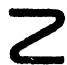
\includegraphics[keepaspectratio]{images/part001_1db83a62.jpg}}

注. 若 X 是局部紧的但不是紧的，则 X 上的闭等价关系 R 未必是豪斯多夫的（第九章，§ 4，习题 14）；而且即使 R 是豪斯多夫的，X/R 也未必是局部紧的（习题 17）。但我们有下述判别准则：

命题 10. 设 X 是局部紧空间，R 是 X 上的一个开的豪斯多夫等价关系，\(f: \mathrm{X} \to \mathrm{X}/\mathrm{R}\) 是典范映射。则 \(\mathrm{X}/\mathrm{R}\) 是局部紧的，且若 \(\mathbf{K}'\) 是 \(\mathrm{X}/\mathrm{R}\) 的任意紧子集，则存在 X 的紧子集 K，使得 \(f(\mathbf{K}) = \mathbf{K}'\)。

第一个断言是如下事实的推论：每个 \(x \in \mathbf{X}\) 有一个紧邻域 \(\mathbf{V}\)，且 \(f(\mathbf{V})\) 是 \(f(x)\) 的一个紧邻域（\(\S 5, \text{no. } 3, \text{ Proposition } 5\) 与 \(\S 9, \text{ no. } 4, \text{ Theorem } 2, \text{ Corollary } 1\)）。对每个 \(y \in \mathbf{K}'\)，设 \(\mathbf{V}(y)\) 是 \(\overline{f}^1(y)\) 的某个点在 \(\mathbf{X}\) 中的一个紧邻域，于是 \(f(\mathbf{V}(y))\) 是 \(y\) 的一个紧邻域。存在有限多个点 \(y_i \in \mathbf{K}'\)，使得诸 \(f(\mathbf{V}(y_i))\) 覆盖 \(\mathbf{K}'\)。设 \(\mathbf{K}_1\) 是紧集 \(\bigcup_i \mathbf{V}(y_i)\)（\(\mathbf{X}\) 中的）；我们有 \(\mathbf{K}' \subset f(\mathbf{K}_1)\)；故 \(\mathbf{K} = \mathbf{K}_1 \cap \overline{f}^1(\mathbf{K}')\) 是紧的（因为它在 \(\mathbf{K}_1\) 中是闭的），且 \(f(\mathbf{K}) = \mathbf{K}'\)。

\section{连通性}
